\documentclass[bachelor,german]{hgbthesis}
% Zulässige Class Options: 
%   Typ der Arbeit: diplom, master (default), bachelor, praktikum 
%   Hauptsprache: german (default), english
%%------------------------------------------------------------

%%% PACKAGES
\usepackage[utf8]{inputenc}
\usepackage[table,xcdraw]{xcolor} % Tabellen

\usepackage[acronym, toc]{glossaries} % Acronym and Glossary

\usepackage{listings} % für inline code definitionen
\definecolor{codestringstylecolor}{rgb}{0.8,0.4,0}
\newcommand\codestringstyle{\color{codestringstylecolor}\ttfamily}
\newcommand\codekeywordstyle{\color{blue}\bfseries}
\lstdefinelanguage{JavaScript}{ % JavaScript definition für listings package
    keywords={typeof, new, true, false, catch, function, return, null, catch, switch, var, if, in, while, do, else, case, break},
    keywordstyle=\codekeywordstyle,
    ndkeywords={class, export, boolean, throw, implements, import, this},
    ndkeywordstyle=\color{darkgray}\bfseries,
    identifierstyle=\color{black},
    sensitive=false,
    comment=[l]{//},
    morecomment=[s]{/*}{*/},
    commentstyle=\color{purple}\ttfamily,
    stringstyle=\codestringstyle,
    morestring=[b]',
    morestring=[b]"
}
\lstdefinelanguage{json}{ % JSON definition für listings package
  stringstyle=\codestringstyle,
  morestring=[b]',
  morestring=[b]"
}

\lstdefinelanguage{yml}{ % YML definition für listings package
  keywords={true,false,null,y,n},
  keywordstyle=\codekeywordstyle,
  %basicstyle=\color{black}\bfseries, this makes the font bigger.
  sensitive=false,
  comment=[l]{\#},
  morecomment=[s]{/*}{*/},
  commentstyle=\color{purple}\ttfamily,
  stringstyle=\codestringstyle,
  moredelim=[l][\color{orange}]{\&},
  moredelim=[l][\color{magenta}]{*},
  moredelim=**[il][\color{red}\mdseries{:}\color{blue}\mdseries]{:},
  morestring=[b]',
  morestring=[b]",
  literate =    {---}{{\llap{\color{cyan}\mdseries-{-}-}}}3
                {>}{{\textcolor{red}\textgreater}}1     
                {|}{{\textcolor{red}\textbar}}1 
                {\ -\ }{{\mdseries\ -\ }}3,
}

%\usepackage{amsmath} % Formeldarstellung

\usepackage{longtable}
\usepackage{booktabs} % Tabellen
\usepackage{multirow} % Tabellen

\usepackage{nameref}

\usepackage[a4paper, total={152.4mm, 223.2mm}]{geometry} % page margin

\usepackage{float} % benutzt für \begin{figure}[H]

%\usepackage{lscape} % für \begin{longtable}

% To strikeout text: 
% example \sout{Hello World}
\usepackage[normalem]{ulem}

% https://www.scribbr.de/apa-standard/verweise-im-text-laut-apa-standard/
% https://tex.stackexchange.com/questions/35809/how-do-i-use-apa-style-citations-with-bibtex#35813
% http://ctan.org/tex-archive/biblio/bibtex/contrib/apacite/
%\usepackage{apacite} % apa style citation
%\bibliographystyle{apacite}
%\bibliography{literatur.bib}


\usepackage{tocbibind}
 % packages importieren

\graphicspath{{images/}}    % wo liegen die Bilder? 
\bibliography{literatur}  	% Angabe der BibTeX-Datei, % utf8-change
\makenoidxglossaries

\newglossaryentry{maths}
{
    name=mathematics,
    description={Mathematics is what mathematicians do}
}

\newacronym{lcm}{LCM}{Least Common Multiple}
\newacronym{IoT}{IoT}{Internet of Things}
\newacronym{DAPP}{DAPP}{Decentralized Application}
\newacronym{DAPPs}{DAPPs}{Decentralized Applications}
\newacronym{EVM}{EVM}{Ethereum Virtual Machine}

% Kolonnen Definition für Tabellen
\newcolumntype{L}[1]{>{\raggedright\arraybackslash}p{#1}} % linksbündig mit Breitenangabe
\newcolumntype{C}[1]{>{\centering\arraybackslash}p{#1}} % zentriert mit Breitenangabe
\newcolumntype{R}[1]{>{\raggedleft\arraybackslash}p{#1}} % rechtsbündig mit Breitenangabe

% Config für tree listings
\lstdefinestyle{tree}{
  literate=
  {├}{{\smash{\raisebox{-1ex}{\rule{1pt}{\baselineskip}}}\raisebox{0.5ex}{\rule{1ex}{1pt}}}}1 
  {─}{{\raisebox{0.5ex}{\rule{1.5ex}{1pt}}}}1 
  {└}{{\smash{\raisebox{0.5ex}{\rule{1pt}{\dimexpr\baselineskip-1.5ex}}}\raisebox{0.5ex}{\rule{1ex}{1pt}}}}1 
}

%%%----------------------------------------------------------
\begin{document}
%%%----------------------------------------------------------

% Einträge für ALLE Arbeiten:
\title{lokkit - Einsatz von Blockchain und IoT}
\author{D.\ Hirzel und A.\ Schmid}
\studiengang{Informatik}
\studienort{Rotkreuz}
%\schulname{Lucerne University of Applied Sciences and Arts}
\schulname{Hochschule Luzern}
\abgabedatum{2017}{06}{09}
%\strictlicense  % erzeugt restriktive Lizenzformel

%%%----------------------------------------------------------
\frontmatter

\maketitle

\tableofcontents
%%%----------------------------------------------------------		

% \include{chapters/02_Selbststaendigkeitserklaerung} wird durch \maketitle bereits gemacht.
\chapter{Abstract d}
\label{cha:abstract_d}

Die \emph{Blockchain}-Technologie ist zurzeit stark im Trend. Sie benutzt verteilte und dezentrale Rechnernetzwerke und bietet dadurch bessere Transparenz und geringere Kosten im Vergleich zu traditionellen Methoden. Auch wird dadurch die Sicherheit erhöht, da die einzelnen Nodes sich gegenseitig versichern, wahrheitsgemäss zu handeln.\cite{BlockchainRevolution}

Pioniert wurde die Blockchain Technologie durch die bekannte bitcoin Blockchain. Neue Blockchain Implementationen unterstützen neben Crypto-Währungen auch sogenannte \emph{Smart Contracts}, die es einem Benutzer erlauben, Programmcode zu implementieren, der in der Blockchain abgelegt wird. Dadurch, dass dieser Code zusammen mit den Daten einsehbar ist, können so Verträge unmissverständlich und öffentlich einsehrbar definiert werden. Programme, die diese Smart Contracts verwenden, nennt man auch \emph{\acrfull{DAPP}}.\cite{BlockchainRevolution}

Auch das Thema \acrshort{IoT} ist seit mehreren Jahren in aller Munde und wächst in den kommenden Jahren stark an. Gartner schätzt einen Zuwachs von 20.4 Milliarden Geräten bis 2020. Dies bringt neue Anforderungen an die Sicherheit mit - ein Aspekt, der eventuell durch die Blockchain-Technologie erfüllt werden kann.\cite{gartner.com_iot,BlockchainRevolution}



\chapter{Abstract d}
\label{cha:abstract_d}

Abstract goes here

%\printglossary[title=Abkürzungen und Definitionen, toctitle=List of terms]

\printnoidxglossary[type=\acronymtype]
 
\printnoidxglossary

%%%----------------------------------------------------------
\mainmatter         % Hauptteil (ab hier arab. Seitenzahlen)
%%%----------------------------------------------------------

\chapter{Aufgabenstellung}
\label{cha:Aufgabenstellung}
\begin{itemize}
    \item \textbf{Grob beschreiben, was erreicht werden soll. Wünsche von Auftraggeber}
    \item \textbf{Eigene Idee und Wünsche erklären. Brainstorming für Ideen auflisten (evtl. Anhang)}
    \item \textbf{lokkit. Konkrete Aufgabenstellung mit use cases, szenarien, business überlegungen (für Hüsler, bspw. möglichen Missbrauch und "kriminelle Energie" erläutern) und requirements. KEINE technischen details, diese folgen im Kapitel Implementation} \ref{sec:Implementation}
    \item \textbf{Erkären warum Wunsch von Auftraggeber erfüllt}
\end{itemize}

Hier folgt die Aufgabenstellung, die ebenfalls im Rahmen dieser Projektarbeit erarbeitet wurde. Einzig die Schlagworte \emph{Blockchain}, \emph{\acrfull{IoT}} und der Bau eines Demonstrators waren vom Auftraggeber im Kick-Off Meeting vorgegeben worden. Im Rahmen dieser Bachelorarbeit sollte ein System definiert, konzipiert und entwickelt werden, das den Blockchain und IoT Aspekt verbindet und einen praktischen Anwendungszweck demonstriert. Der entwickelte Demonstrator sollte nach Abschluss dieses Projektes noch weiter vom Auftraggeber als solcher verwendet werden können.

\section{Ziele}
\label{sec:Ziele}
"Der zentrale Aspekt dieses Projektes war der Wissenserwerb im Bereich Blockchain und die konkrete Anwendung dieses neu erworbenen Wissens durch die Konzeption und Implementation eines IoT Demonstrators. Dieser sollte durch sorgfältige und gründliche Arbeit dem Auftraggeber in einem eigenständig verwendbaren Zustand übergeben werden können. Die konkrete Aufgabenstellung für den Demonstrator wurde ebenfalls im Rahmen dieses Projektes vom Projektteam entwickelt und mit dem Auftraggeber besprochen", \ref{pm_subsec:Projektziele}.

\section{Konkrete Aufgabenstellung}
\label{sec:Konkrete_Aufgabenstellung}
\emph{Da die konkrete Aufgabenstellung in dieser Bachelorarbeit ebenfalls erarbeitet werden musste, ist diese ein Produkt der Recherchephase (vgl. \ref{pm_subsubsec:Recherchephase}). Bei fehlendem Wissen um Blockchain, Ethereum oder den entwickelten Demonstrator wird empfohlen, die einleitenden Kapitel der Lösungsfindung \ref{sec:Arbeitsmethodik} und \ref{sec:Recherche} vorzugreifen.}

Es soll ein System entwickelt werden, um Schliessfächer zu (ver-)mieten. Dabei sollen die Verträge in Form von Smart Contracts (vgl. \ref{subsec:Recherche_Smart_Contracts}) in einer privaten Ethereum Blockchain (vgl. \ref{subsec:private_chain}) definiert werden. Ein Benutzer soll über eine grafische Benutzeroberfläche ein freies Schliessfach reservieren können. Während der Benutzer der aktuelle Mieter eines Faches ist, kann er das Schloss per Knopfdruck ver- und entriegeln.

\section{Anforderungen an den Demonstrator}
\label{sec:Anforderungen_Demonstrator}

\subsection{Smart Contracts}
Die Businesslogik und Datenhaltung ist mittels Smart Contracts zu lösen. Diese bilden das zentrale Objekt in diesem System.

X. Die Smart Contracts sollen eine Funktion bieten, neue Schliessfächer erfassen zu können.

X. Die Smart Contracts sollen eine Funktion zum Eingehen eines zeitlich begrenzten Mietvertrags anbieten.

X. Die Smart Contracts soll Kosten für die Dauer des Mietvertrags definieren, die durch die Überweisung von Ether beglichen werden.

//X. Der Benutzer soll ein Depot für die Mietdauer an die Smart Contracts entrichten, das dem Besitzer eines Schliessfaches als Sicherheit dient, falls das Schliessfach nicht freigegeben wird.

\subsection{Webapp}
Die Interaktion von Benutzern mit Smart Contracts in der Blockchain wird durch eine Webapp umgesetzt. Folgende Anforderungen beziehen sich auf zu entwickelnde Webapp.\cite[Wiki/DAPP-Developer-Resources, Wiki/Useful-Dapp-Patterns]{github.com/ethereum}

X. Die Webapp soll eine Liste von verfügbaren Schliessfächer anzeigen.

X. Die Webapp soll das einfache Hinzufügen von Schliessfächern zu der Liste der verfügbaren Schliessfächern ermöglichen.

X. Die Webapp soll das Mieten von Schliessfächern mit einer einfach zu bedienenden Benutzeroberfläche ermöglichen.

//X. Die Webapp soll dem Benutzer in allen Fällen Rückmeldung über ausgeführte Funktionen geben.

X. Die Webapp soll auf der zur Verfügung gestellten Hardware gehostet werden können (namentlich: Raspi)

\subsection{Mobile App}
Folgende Anforderungen beschränken sich auf die Mobile App für Android (später: Android App).

X. Die Mobile App soll eine Ethereum Node starten, die mit dem definierten privaten Netzwerk verbindet und die verwendet werden, um die Webapp lokal mit der Node zu verbinden.

X. Die Mobile App soll die Erstellung von einem Benutzerkonto auf der lokalen Ethereum Node ermöglichen.

X. Die Mobile App soll...

\subsection{IoT Controller}
Damit die Schliessfächer angesprochen werden können, müssen auf den IoT Geräten Controller implementiert werden, die die Hardware ansteuern. Folgende Anforderungen gelten für alle Controller unterschiedlicher Hardware.

X. Der Controller soll auf gültige Anfragen das Schliessfach öffnen oder schliessen.

\subsection{Demonstrator Hardware}


X. Der Demonstrator soll ohne externe Abhängigkeiten funktionsfähig sein.

X. Der Demonstrator soll...

\subsection{Übergreifend}
Diese Anforderungen sind funktionsübergreifend gültig und müssen von allen betroffenen Komponenten berücksichtigt werden.

X. Ver- und Entriegeln eines Schliessfachs kann nur von einem durch einen Smart Contract berechtigten Benutzer erfolgen.

X. Alle Implementationen mit grafischer Benutzeroberfläche sollen in einem einheitlichen Erscheinungsbild erstellt werden.

\subsection{Scopeabgrenzung}
X. Das Hinzufügen von neuen mietbaren Objekten ist nicht Teil dieser Arbeit. Der Demonstrator wird mit den mitgelieferten Schliessfächern vorkonfigurierten.

X. Die Verwendung von Oracles ist nicht Teil dieses Projekts. Als Oracle wird die Möglichkeit bezeichnet, Berechnungen eines Smart Contracts, durch Verteilung auf mehrere externe Systeme, von der Blockchain zu lösen. Dies ist noch immer ein low-trust Szenario, da keinem externen System alleine die Möglichkeit zur Veränderung der Blockchain gegeben wird, sondern auch der Konsens dieser Systeme in die Blockchain geschrieben wird.\cite{blog.ethereum.org/oracles}

aus einem Smart Conract heraus Systeme anzusprechen, die nicht auf der Blockchain funktionieren. Beispielsweise existieren 

\section{Erwartete Resultate}
\label{sec:Erwartete_Resultate}

\subsection{Software}
\begin{itemize}
    \item Smart Contracts in Solidity
    \item Webapp (Plattformunabhängig)
    \item Mobile App (Android exkl.)
    \item IoT Controllers
\end{itemize}

\subsection{Hardware}
\begin{itemize}
    \item Ein lauffähiger Demonstrator für das Schliessfachsystem.
\end{itemize}

\chapter{Lösungsentwicklung}
\label{cha:Lösungsentwicklung}
Um eine Lösung zu dieser 

\section{Arbeitsmethodik}
Da in diesem Projekt eine konkrete Aufgabenstellung selbst zu erarbeiten war, und keine konkreten, lieferbaren Objekte vorgesehen waren, wurde zu Beginn eine explorative ad-hoc Methodik verfolgt. Dabei wurde im Projektteam wöchentlich der bisherige Fortschritt analysiert und weitergehende Schritte besprochen. So wurde gewährleistet, dass in der Anfangsphase eine geeignete Aufgabenstellung gefunden werden kann.
\par
Sobald die Aufgabenstellung gefunden wurde, wurde in ein iterativ- inkrementelles Modell gewechselt. Die wöchentlichen Besprechungen wurden beibehalten, um den Fortschritt des Produkts zu verfolgen.

\section{Systemübersicht IoT}
\label{sec:Setup_IoT}
Übersicht: Raspis, Schliessfächer etc...
\begin{figure}
\centering
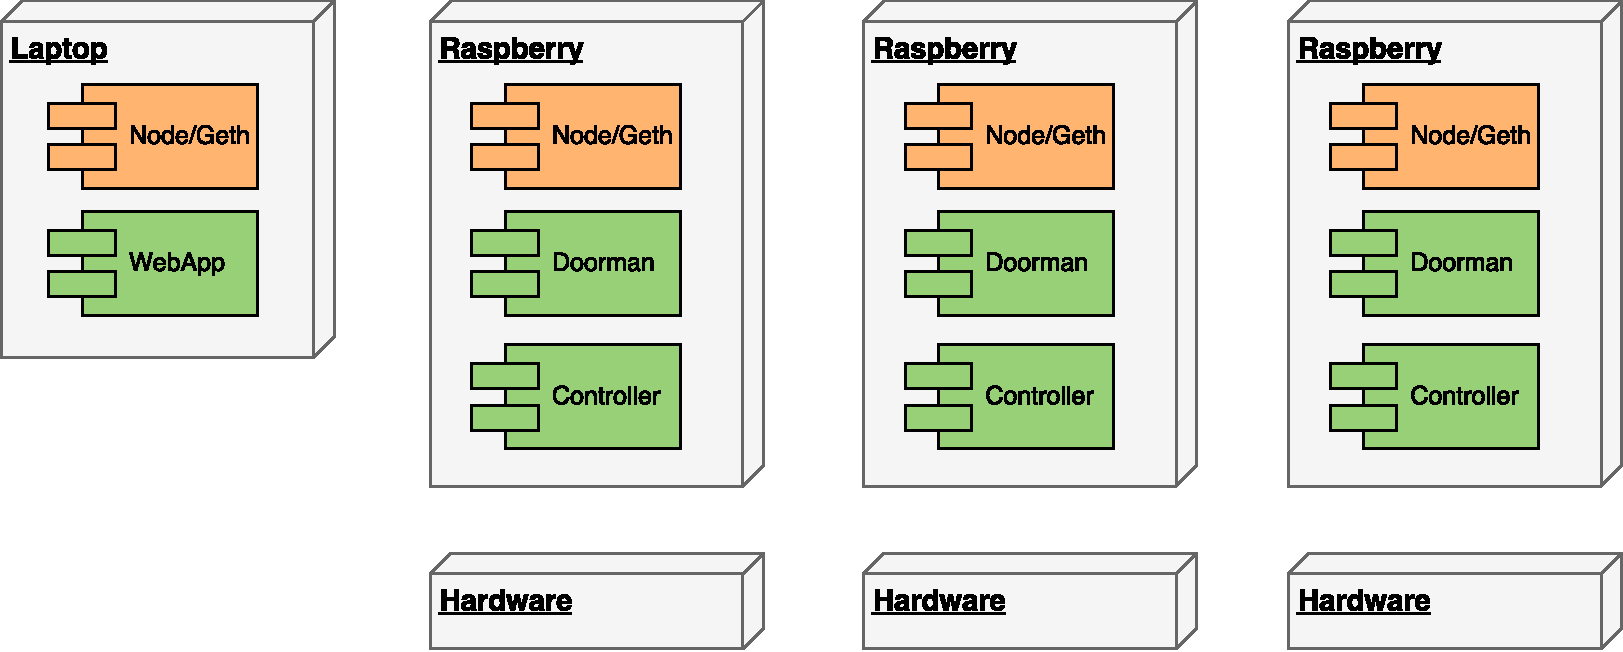
\includegraphics[width=.95\textwidth]{Aufbau_Komponenten} %{CS0031}
\caption{Komponenten und Schnittstellen}
\label{fig:Komponenten und Schnittstellen}
\end{figure}
\subsection{Systemkontext}

\subsection{Systemkomponenten}

\begin{figure}
\centering
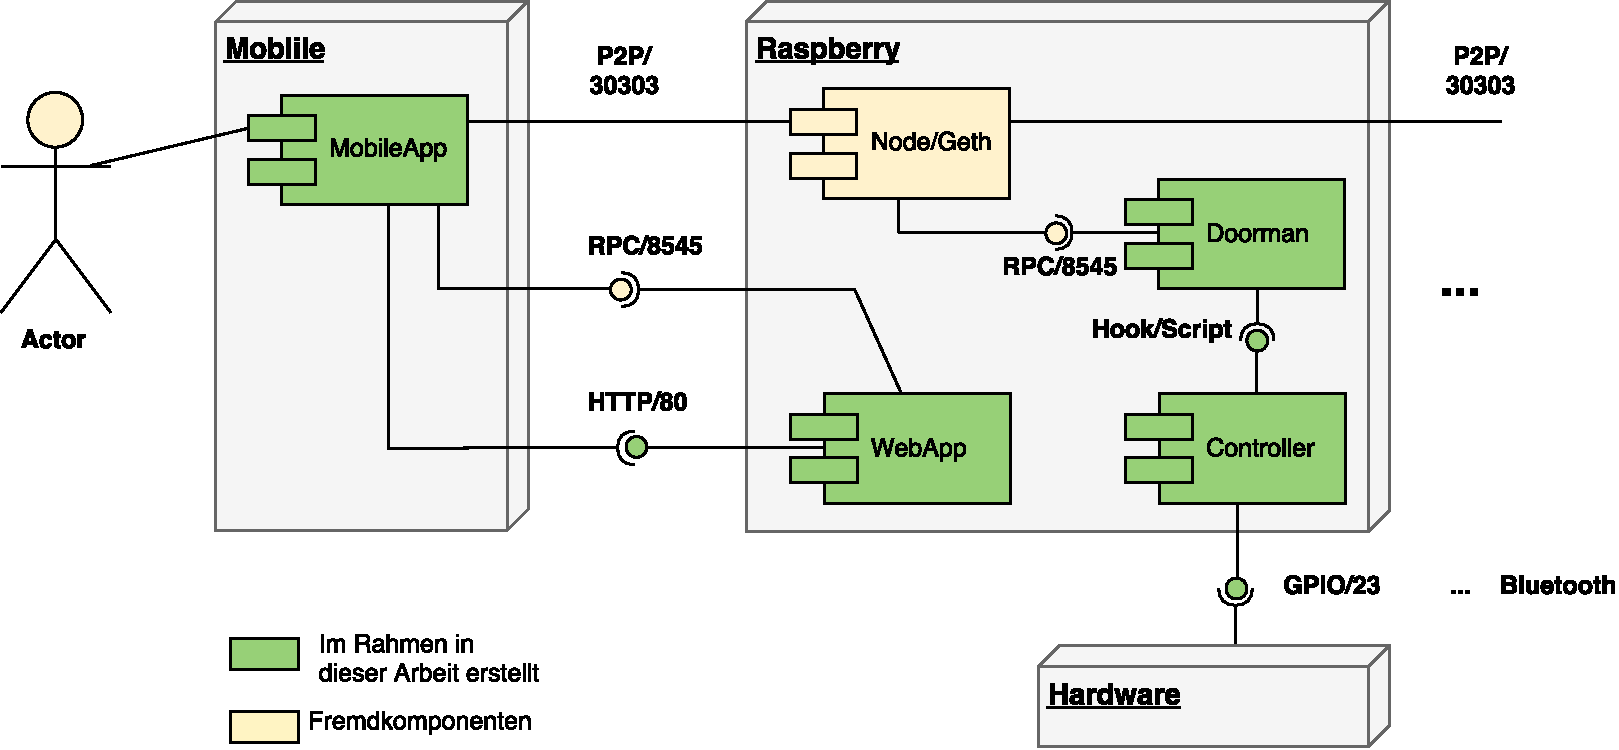
\includegraphics[width=.95\textwidth]{Aufbau_Komponenten_Interface} %{CS0031}
\caption{Komponenten und Schnittstellen}
\label{fig:Komponenten und Schnittstellen}
\end{figure}



\section{Blockchain}
\label{sec:Blockchain}
referenz, verweise

\subsection{Verwendete Implementation}
Wieso Ethereum?

\subsubsection{Ethereum}
\paragraph{Ledger?}
\paragraph{Solidity}
\paragraph{Whisper}
\subsubsection{IBM Hyperledger}
\paragraph{Fabric}
\paragraph{Chaintool}

\subsection{Testchain}

\subsection{Private chain mit Ethereum}


\subsection{Smart Contracts}
\label{subsec:Smart_Contracts}
\epigraph{''A computerized transaction protocol that executes the terms of a contract.``} \cite{BlockchainRevolution}
\\Mit diesem Zitat kann grob das Ziel von Smart Contracts beschrieben werden. Verträge, die in einem maschinenlesbaren Format verfasst sind, können mit unmissverständlicher Präzision und ohne Interpretationsspielraum definiert werden. So ist es möglich, einen deterministischen, digitalen Vertrag zu verfassen.
Entgegengesetzt ist es nahezu unmöglich eine Menge von Smart Contracts angesichts einer unüblichen Situation deterministisch abzuarbeiten. -> http://www.ibtimes.co.uk/pwc-blockchain-expert-pinpoints-sources-ambiguity-smart-contracts-1575778

\susubsection{Erstellen}
Um einen Smart Contract zu erstellen, wird mittels einer geeigneten Programmiersprache dieser formell definiert. Dieser geschriebene Programmcode kann mittels einer Transaktion in die Blockchain eingesetzt werden, wobei Initialwerte angegeben werden. Man sprich hierbei vom erstellen einer Instanz des Smart Contracts, ähnlich wie in der objektorientierten Programmierung. Bei der ausgelösten Transaktion gilt es zu beachten, dass diese keinen Empfänger hat; der Empfänger dieser Nachricht ist die Blockchain selbst. Wie bei jeder Transaktion eine gewisse Menge gas mitgegeben werden, damit die Operation abgeschlossen werden kann. Wenn der Code in die Blockchain eingesetzt wurde, erhält diese Instanz des Contracts eine Adresse, über die später mit dieser spezifischen Instanz interagiert werden kann.
Beim Erstellen eines Smart Contracts wird auch ein abi generiert. Dieses beschreibt die möglichen verfügbaren Attribute des Contracts und die Interaktionsmöglichkeiten (\#VGL. Funktionen) inklusive deren allfällige Parameter und Rückgabewerte (\#VGL. Interfacedeklaration in OO Sprachen).

\susubsection{Lesezugriff}
Um ein Attribut auszulesen oder eine Funktion mit konstantem Rückgabewert auszuführen, kann diese über ein verfügbares Interface, wie die JavaScript console von geth, direkt aufgerufen werden. Bei Funktionen mit konstantem Rückgabewert ist zu beachten, dass diese nur auf der lokalen Node emuliert werden (CITATION NEEDED) und es somit nicht möglich ist, eine Änderung in der Blockchain zu bewirken. Diese Funktionen haben folglich nur Lesezugriff.

\subsubsection{Schreibzugriff}
Wenn eine Funktion auf der Instanz aufgerufen wird, die eine Änderung in der Blockchain bewirkt, muss eine Transaktion ausgelöst werden. Der Sender der Transaktion muss dabei für die Kosten für gas und allfällige weitere Kosten (\#VGL. Bezahlbare Funktionen) aufkommen. Der Sender kann nicht nur ein Account sein, sondern auch ein weiterer Smart Contract, an dessen Adresse genügend Ether liegt, um die Transaktionskosten zu begleichen.

\paragraph{Bezahlbare Funktionen}
Einige Funktionen benötigen mehr Ether als nur die gas-Kosten. Wenn beispielsweise eine Dienstleistung oder Sache über einen Smart Contract verkauft werden soll, muss noch eine Menge Ether als Zahlungsmittel überweisen werden. Die Menge Ether ist im Smart Contract festgelegt und kann durch Inspektion des Programmcodes eingesehen werden. Sollte der Kunde zu wenig Ether schicken, kann der Smart Contract definieren, dass die Transaktion nicht erfolgreich ist und der Kunde sein Geld zurückerhält. Dazu kann die Transaktion selbst als nichtig erklärt werden und es muss nicht auf das Withdrawal Muster zuückgegriffen werden.

\subsubsection{Solidity}
Solidity ist eine Programmiersprache zur Erstellung von Smart Contracts auf der \acrfull{EVM}, die syntaktisch stark an JavaScript angelehnt ist. Sie kann auch auf anderen Blockchain Platoformen (wie Tendermint oder Counterparty für Bitcoin) verwendet werden. -> https://www.cryptocoinsnews.com/counterparty-brings-ethereum-smart-contracts-to-the-bitcoin-blockchain/\\Solidity wird, in Anlehnung auf den Ausdruck object-oriented, als contract-oriented beschrieben, da die erstellenden Konstrukte in der Sprache als ''contract`` und nicht ''object`` bezeichnet werden. Inhaltlich beziehen sich die beiden Ausdrücke auf dasselbe Konzept.

\subsubsection{Gängige Muster - GEHÖRT DAS INS KAPITEL "SMART CONTRACTS" ODER HIERHIN?}
Folgend werden einige Muster aufgelistet, die beim Entwurf und der Implementation von Smart Contracts mit Solidity, aufgrund der inhärenten Architektur der Platform und Sprache, beachtet werden sollten. Diese Muster dienen als Richtlinie und umgehen bekannte Limitationen oder schliessen Sicherheitslücken. Es ist möglich unter Misachtung der Muster Smart Contracts zu entwickeln. -> \#ALLE BEISPIELE VON http://solidity.readthedocs.io/en/develop/
\#Alle folgenden Beispiele waren für die Erarbeitung der Rentable \& RentableDiscovery Contracts zu beachten!

\paragraph{Generell}
Instanzen von Smart Contracts erhalten, wie Accounts, ebenfalls eine Adresse, an die Ether geschickt werden kann. Meistens wird dies in Form von Funktionsaufrufen gemacht, allerdings kann auch direkt an einen Smart Contract Ether überwiesen werden. Hierbei ist es wichtig zu beachten, dass der Ether zurückerstattet wird, der aus Veresehen an diesen gesendet wurde (\#VGL Withdrawal Muster).

\paragraph{Withdrawal Muster}
Wenn aus einem Smart Contract eine Transaktion an eine Adresse gestartet wird, muss das gas dafür vom digitalen Vertrag bezahlt werden (oder besser: vom Account, der die ursprüngliche Transaktion an den ersten digitalen Vertrag gestartet hat). Im Fall einer einfachen Überweisung fallen keine gas-Kosten an. Ist das Ziel aber ein anderer Smart Contract, besteht die Möglichkeit, dass der Zielvertrag Code ausführt, wenn er eine Transaktion erhält. Das Withdrawal Muster wird folglich verwendet, um zu verhindern, dass der Quellvertrag dies überprüfen muss oder für die gas-Kosten des anderen Smart contracts aufkommen muss.

Wird das Withdrawal Muster angewendet, überweist ein Smart Contract Ether nicht direkt an eine Zieladresse. Stattdessen merkt er sich die Menge, die einer Zieladresse zusteht und stellt die Möglichkeit zur Verfügung, dass diese Begünstigten Ether abheben können. Dies findet mittels einer Transaction statt, die vom Begünstigten ausgelöst werden muss. Die gas-Kosten für diese Art Funktionen sind meist vernachlässigbar und werden durch die zurückerhaltene Menge Ether kompensiert. Da der Begünstigte die Adresse des Quellvertrags kennt und den Quellcode von Smart Contracts öffentlich ist, kann die Zieladresse sicher gehen, beim aufrufen dieser withdrawal-Funktion auf dem Quellvertrag auch tatsächlich die Menge Ether zurückzuerhalten.
http://solidity.readthedocs.io/en/develop/common-patterns.html\#withdrawal-from-contracts

\#möglicherweise ein bildli zeichnen oder beispielcode einfügen


\paragraph{Re-Entrancy}
Hierbei handelt es sich um ein Muster, das angewendet wird, wenn in einem Smart Contract A ein interner Zustand existiert, der die Menge an Ether speichert, der \emph{anderen} zusteht und eine Möglichkeit besteht, diese Menge Ether zu entnehmen (\#VGL. Withdrawal Muster). Beispiele für zurückzuerstattenden Ether kann ein Gebot in einer Auktion sein oder Depots wie bei lokkit.
Unter der Annahme, dass die Zieladresse für die Rückerstattung ein Smart Contract B ist, kann B A angreifen. Bei einer Transaktion wird immer der zugehörige Code ausgeführt. Das heisst, dass B auf eine eingehende Transaktion reagieren kann und ihrerseits erneut die Transaktionsfunktion von A aktivieren kann (\#VGL. Withdrawal Muster). Wenn der Zustand von A noch nicht geändert wurde, wird der Betrag erneut gesendet, bis A kein Ether mehr zur Verfügung hat.

Um mehrfaches Überweisen von Ether zu verhindern, ist es essentiell, zuerst den internen Status des Vertrags zu ändern, bevor Ether überwiesen wird. Die \emph{total} zur Verfügung stehende Menge Ether eines Smart Contracts wird in der Blockchain gehalten und ist Teil des Konsensus. Es ist somit nicht möglich, dass mehr Ether ausgegeben wird als in dem jeweiligen digitalen Vertrag vorhanden ist. 

CODE SNIPPET FALSCH:
    function withdraw() {
        if (msg.sender.send(deposit[msg.sender])) { // das kann mehrere male ausgeführt werden.
            deposit[msg.sender] = 0;
        }
    }
CODE SNIPPET RICHTIG:
    function withdraw() {
        var currentRefund = deposit[msg.sender]; // zurückerstattend Menge auslesen
        deposit[msg.sender] = 0; // momentanes Depot zurücksetzen, bevor überwiesen wird! Dies wehrt die Re-Entrancy Attacke ab
        msg.sender.transfer(currentRefund); // hier transfer anstatt send benutzen, da (\#TODO)
    }

http://solidity.readthedocs.io/en/develop/security-considerations.html\#re-entrancy

\section{Komponenten}
\label{sec:Komponenten}
Nachfolgend werden die einzelnen Komponenten beschrieben, die für die volle Funktionalität der lokkit-Philosophie benötigt werden.
\subsection{Doorman}
Doorman implementiert die IoT-Seite der Benachrichtigungen mitterls Whisper Protokoll.
\subsubsection{Wieso Python? Wieso Python 2.7?}
\subsubsection{Mechanismus}

\subsection{Smart Contracts (Business Logik)}
Die Smart Contracts, die mit Solidity implementiert wurden, werden nachfolgend erläutert. Diese Smart Contracts bilden das Rückgrat der Applikation und bilden die Business Logik in Code Form ab und legen sich als Zugriffslayer zwischen die Userinteraktion und die Blockchain als Datenbank.

\#WICHTIG!!
Erwähnen der shortcomings, da unsere Contracts eine nicht vordefinierte Anzahl Iterationen haben. Dies kann aufgrund des Block-Gas limits zu stalling führen. Auch lese-Operationen, die aus anderen Smart-Contracts aufgerufen werden können diesen zum stallen bringen. -> http://solidity.readthedocs.io/en/develop/security-considerations.html\#gas-limit-and-loops

\subsubsection{Rentable}
\subsubsection{RentableDiscovery}

\subsubsection{Weitere Überlegungen}
noch einen separaten "data-store" für die Reservationen. Nicht-beachtete Konzepte. Raum für Verbesserungen.


\subsection{Frontend}
\subsubsection{Mobile App (Android)}
\paragraph{geth / offizielle API}
\paragraph{Status.io}
mit Verweis auf Testchain

\subsubsection{DApp}
\paragraph{Embark}
\paragraph{Vue.js}

\subsubsection{Command Line Client (geth attach)}


\section{}
\chapter{Schlussfolgerung}
\label{cha:Schlussfolgerung}

Abschliessend wird über das Projekt und dessen Ablauf reflektiert. Die erledigte Arbeit wird folgend infrage gestellt und eine kritische Position gegenüber der verwendeten Technologien, Entscheidungen im Projektverlauf und der Aufgabenstellung angenommen.

\section{Fazit Aufgabenstellung}
\label{sec:Fazit_Aufgabenstellung}
Die Umsetzung der erarbeiteten Aufgabenstellung dient als Demonstrator und soll ein \acrfull{PoC} sein. Der Fokus war von Anfang an, auch seitens der Auftraggebers, auf der Blockchain Technologie. Der \acrshort{IoT} Aspekt sollte der abschliessenden Veranschaulichung des \acrshort{PoC} dienen. Dabei gab es einige Limitationen in der Anwendung der Funktionalitäten der Blockchain, da auf die Komplexität und die Anwendungsbereiche der zu implementierenden Demonstrator Hardware Rücksicht genommen werden musste. Die physische Umsetzung des Demonstrators hat auch Zeit gekostet, die anders verwendet zu zusätzlichen Erkenntnissen im Bereich Blockchain hätte führen können.

Der unmittelbare Nutzen des Demonstrators, wo zentrale Angebote bereits vorhanden sind, beispielsweise an Bahnhöfen der SBB, ist nicht sofort ersichtlich. Einige Nachteile in diesem konkreten Beispiel wären benötigte Elektronik, Stromverbrauch und Verfügbarkeit des Angebots. Auch die Abhängigkeit zu der Blockchain kann verheerende Folgen haben, sollte dieses aus einem beliebigen Grund kompromittiert werden.

Das System wurde nur im Rahmen eines privaten Netzwerkes aufgebaut und getestet - kurze explorative Exkurse auf die \emph{Ropsten} Testchain sind davon ausgeschlossen. Skalierungsfragen wurden hierbei nicht beantwortet, wie beispielsweise die Performance und Zuverlässigkeit der Events aus Solidity oder Propagation von Whisper v5 Nachrichten in der öffentlichen Blockchain. Sollte erhebliche Latenz durch die Skalierung entstehen, wäre die Lösung so nicht zu verwenden und würde die Kundenzufriedenheit negativ beeinflussen.

\section{Fazit Blockchain}
Wie im Kapitel \ref{sec:Fazit_Aufgabenstellung} erwähnt, konnte aufgrund der Aufgabenstellung nicht alle Zeit in diesem Projekt in die Aufbereitung und Anwendung der Blockchain Technologie investiert werden. Trotzdem wurde ein Einblick in dieses Thema gewährt, der einen bleibenden Eindruck hinterliess.

Ein grosser Aspekt der Blockchain ist Anonymität und Vertrauenslosigkeit. Wie Schächen zu Stärken werden können, kann dies auch umgekehrt der Fall sein: Genau diese beiden Punkte werden zum Verhängnis, wenn konkrete Dienste angeboten werden sollen. An dieser Stelle sind Organisationen wie Silk Road\footnote{https://en.wikipedia.org/wiki/Silk\_Road\_(marketplace)} zu erwähnen, die im Angesicht solcher Technologien auf den Plan gerufen werden. Auch aufgrund des mangelnden Vertrauensverhältnisses zwischen Dienstleister und dem, der den Dienst bezieht, muss auf Vorsicht beharrt werden, falls Dienste in der realen Welt oder physische Produkte auf Bezahlung mit Kryptowährungen ausgetauscht werden.

\subsection{Fazit Ethereum}
Durch die Mitarbeit an dem Open Source Projekt go-ethereum wurde klar, dass das Ethereum Protokoll und auch die Umsetzung in geth trotz mehrjähriger Entwicklung noch lange keinen finalen Stand erreicht hat. Grundlegende Diskussion zum Design des Protokolls und dessen Implementation werden in den Kommunikationskanälen rege vorangetrieben.\cite[Gitter]{go-ethereum}

\section{Fazit Blockchain und IoT}
Das Konzept der Rentables wurde bewusst so abstrakt gewählt, um die Ausdehnung zu ermöglichen. Ein Rentable kann dabei grundsätzlich alles sein: Ein elektrisches Fahrrad, eine Ferienwohnung oder ein Schliessfach. Es muss jedoch möglich sein, einen Kontrollmechanismus anzubringen, der an eine Blockchain Node angebunden werden kann. Bei einem elektrischen Fahrrad wäre es z.B. möglich einen Minicomputer im Fahrgestellt zu montieren, welcher den Akku aktiviert oder deaktiviert und über eine Sim-Karte mit der Blockchain synchronisiert. Möchte ein Benutzer das Fahrrad verwenden, so müsste er dieses zuerst über die Blockchain mieten und erst dann kann er den Akku aktivieren. Die Mietkosten würden über den Smart Contract dem Anbieter des Fahrrades überwiesen werden.

\section{Ausblick}
Aufbauend auf diesem Demonstrator, dieser Arbeit und den Erkenntnissen daraus, könnte vom Auftraggeber Nutzen gezogen werden. Die weitere Verfolgung dieses Konzeptes könnte, unter Beachtung der weiteren Überlegungen im Bereich der Smart Contracts (vgl. \ref{para:Rentable_weitergehend}), verfeinert werden, und an Firmen demonstriert werden, um das noch vorhandene Mysterium um diese Smart Contracts in der Blockchain zu lüften.

\section{Lessons Learned}
\label{sec:Lessons_Learned}
Hier schreiben die Diplomanden ihre abschliessenden Worte zur Bachelorarbeit.

\subsection{Dominik Hirzel}
Das war das interessanteste und lehrreichste Projekt, an dem ich im schulischen und professionellen Umfeld je gearbeitet habe. Nie wollte ich mit einem meiner Kommilitonen tauschen. Diese Aussage dient nicht dazu, eine bessere Note ergaunern zu wollen, sondern soll vielmehr dazu meine Euphorie sowie meinen Arbeits- und Lernwillen in diesem Projekt auszudrücken. Einen grossen Teil dieser Motivation und Ausdauer verdanke ich auch meinem technisch wie sozial ausserordentlich versierten Partner: Andreas Schmid (vgl. \ref{andi}).

Die cutting edge Technologie der Blockchain interdisziplinär mit dem IoT Aspekt zu verbinden hat mir nicht nur schlaflose Nächte und eine Bekanntschaft mit dem Nachtwächter der HSLU beschert, sondern auch viele Freudensprünge erlaubt. Dieses Projekt hat mich in meiner Entscheidung bekräftigt, nach wie vor die passende Ausbildung und das passende Studium gewählt zu haben.

Speziell die Zusammenarbeit mit den Open Source Projekten Ethereum und Status-IM hat mir gefallen. Die Tatsache, dass wir ihnen in ihrem Design und der Implementation Fehler gefunden haben und diese mitteilen konnten (vgl. \ref{subsec:Open_Source}) bestätigt auch die Intensivität und unser Engagement in dieser Arbeit.

Die unterschiedlichen entworfenen Softwarekomponenten und das Zusammenspiel dieser, sowie das Design der Real-Time Kommunikationsschnittstelle und Berücksichtigung der Sicherheitsrelevanten Aspekte, waren aus technischer Sicht ein Highlight dieser Arbeit. Allgemein lässt sich die Komplexität dieses Systems betonen, das wir mit klar abgegrenzten Verantwortungsbereichen entworfen und umgesetzt haben.

\subsection{Andreas Schmid}
\label{andi}
Es bereitete mir Freude, mich mit meinem Kameraden in die weiten Abgründe der Blockchain und deren Smart Contracts zu stürzen. Gerade jetzt, wo das Thema brandaktuell ist und viele namhafte Firmen damit am Experimentieren sind, sind wir doch eines der ersten Teams, das einen funktionierenden und anfassbaren Demonstrator gebaut hat. Der Weg war holprig und nicht immer einfach und doch sind wir motiviert und erfolgreich am Ball geblieben. Herzlichen Dank an dieser Stelle an meinen kompetenten und ambitionierten Mitstreiter Dominik Hirzel.

Auch nach dieser sehr intensiven und aufregenden Zeit voller Überstunden und kurzen Nächten, ist mein Wissensdurst noch nicht gestillt und viele Fragen stehen noch offen. Diese Thematik wird mich sicherlich noch weiter beschäftigen.

Einmal mehr bin ich davon überzeugt, dass Open Source Projekte der richtige Ansatz für Software Engineering ist. Nur so kann die Zusammenarbeit über Projekte hinweg gefördert und weltbewegende Software geschrieben werden. Wir sind während dieser Arbeit stark in Kontakt mit den Entwicklern von Ethereum und Umsystemen geraten und haben sowohl für uns wie auch für die Community einen Nutzen generieren können.

Ich bin nach wie vor überzeugt, im richtigen Umfeld tätig zu sein und freue mich bereits auf die nächste Herausforderung. 


%\include{chapters/09_Quellen_Tabellen_Abbildungsverzeichnisse}
%%%----------------------------------------------------------
%%%Anhang
\appendix
%\chapter{Arbeit mit Open Source Projekten}
\label{app:Open_Source}
Hier wird die Verwendung der Open Source Projekten inkl. Anwendungsspezifischer Änderungen für das lokkit Projekt gelistet.

\section{https://github.com/ethereum/go-ethereum}
\label{app:sec:Go_Ethereum}
geth ist supi

\section{https://github.com/status-im/status-go}
\label{app:sec:Status_Go}
status-go wurde geforkt, da die Config für die mainnet und testchains statisch eingebunden wurde. ohne diese Änderung wäre es nicht möglich gewesen eine node auf einem mobilen gerät auf eine private blockchain zu connecten.

\section{weitere?}
\label{app:sec:XXXXX}
\begin{itemize}
    \item{evtl npm/truffle/embark?}
    \item \textbf{some txt}
\end{itemize}
\chapter{Alte Ideen}

\section{Überarbeitet}

\subsection{Real-Time Kommunikationsschnittstelle Whisper v2}
Um mit mietbaren Objekten (vgl. \ref{subsec:lokkit_Smart_Contracts}) während des gemieteten Zeitraums in Echtzeit zu interagieren, wurde das Whisper Protokoll (vgl. \ref{para:Whisper}) verwendet. Whisper erlaubt nur die Übermittlung von einfachen testbasierten Nachrichten. In dieser Schnittstelle definiert wurde eine Nachricht im JSON Format\footnote{http://json.org/}, die eine strukturierte Möglichkeit zur Datenüberittlung ermöglicht.
Die Nachricht selbst besteht aus einem einzelnen JSON Objekt. Dieses Objekt besitzt zwei Attribute: \emph{digest} (vgl. \ref{para:Digest}) und \emph{message} (vgl. \ref{para:Message}).

\begin{lstlisting}[language=json,caption={Beispiel einer Real-Time Nachricht via Whisper Protokoll}]
{
  digest: "0xf88a8a19e428f25f6489aae44c09f2e142297a4053a8aaef5a97c4c2b246c89477"
    + "a2fc16365a0ec05a466e23b403ac1370eedc5e90032ca007d742edfad83eb11b",
  message: {
    command: "open",
    rentableAddress: "0x4cbee4df58c717f47a5e6e8d305a450fcdbe1e24",
    whisperIdentity: "0x04eee314d1b1a4e9f264055274d7411200ada940d6c6c698d53bf40b41ff0f5277"
    + "75a8dfd11867fe64d389ab7cb9809f8df08f561a2498fdd9c9d5c6556913f598"
  }
}
\end{lstlisting}

\paragraph{Message}
Das Message Objekt innerhalb der Nachricht enthält drei Attribute: command, rentableAddress und whisperIdentity. Dies ist die primäre Mitteilung, die an ein IoT Gerät gemacht werden möchte.
\subparagraph{Command}
Dieses Command verkörpert den Befehl, der ausgeführt werden soll. Abhängig von der jeweiligen Implementation des IoT Geräts kann dieses Command etwas anderes beinhalten. Standardmässig werden \emph{open} und \emph{close} für Schliessfächer geschickt.
\subparagraph{Rentable Address}
Obwohl die Adresse bereits in den topics der Nachricht vorhanden ist, wird sie in der Message erneut angegeben. Grund dafür ist, dass die topics nur der Filterung der Nachrichten dienen. Das Message Objekt wurde kryptographisch signiert und somit kann festgestellt werden, dass die Nachricht auch wie gesendet zugestellt wird.
\subparagraph{Whisper Identity}
Obwohl die Whisper Identity optional für Whisper ist (vgl. \ref{old_supara:Whisper_Identity}), wird sie vorausgesetzt, um die Real-Time Kommunikation von lokkit zu benutzen. Die Whisper Identity des Absenders einer Nachricht ist öffentlich zugänglich und kann von jeder Nachricht abgefragt werden, sofern ein Absender gesetzt wurde.

\paragraph{Digest}
Whisper Nahrichten kann ein Sender und ein Empfänger in Form von \emph{Whisper Identities} angegeben werden. Da diese Whisper Identities aber nicht an Adressen in der Blockchain gebunden, sondern kurzlebige Objekte sind, wurde eine weitere Sicherheitsmassnahme implementiert, um den korrekten Absender einer Nachricht zu validieren.
Zusätzlich zu der in Whisper vorhandenen Möglichkeit Sender und Empfänger einer Nachricht anzugeben, wurde eine in der web3 enthaltene Funktion \emph{web3.eth.sign(...)} verwendet, um die übermittelte Nachricht zu signieren. Damit diese Funktion einen Wert zurückliefert, muss der Private Key des angegebenen Accounts auf der lokalen Node vorhanden sein und dieser Account muss über die Funktion web3.personal.unlockAccount(...) entsperrt sein. Sind diese Vorbedingungen erfüllt, liefert \emph{web3.eth.sign(...)} eine 130-Stellige HEX-Zahl zurück.

Wichtig bei web3.eth.sign(...) ist, dass die über Whisper erhaltenen JSON Objekte jeweils die Attribute in alphabetisch sortierter Reihenfolge beinhalten und über die javascript Funktion JSON.stringify serialisiert werden, bevor sie den kryptographischen Funtionen übergeben werden. Grund dafür ist, dass besagte sign Funktion eine Zeichenkette als Arugment nimmt und nicht ein Objekt. Die Verwendung von JSON.stringify versichert, dass der eingabewert stets gleich strukturiert ist.

\paragraph{Replay Attack}
Sollte die Whisper Identity nicht Teil der signierten Message sein, könnte ein Angreifer eine Replay Attacke ausführen, indem dieselbe Nachricht erneut versendet wird. Als Alternative zur Einbettung der Whisper Identity im signierten Message Objekt könnte zur Verhinderung dieser Attacke die empfangende Whisper Identity im Smart Contract Rentable angegeben werden. Die Erstellung eines Absenders würde somit obsolet und Whisper würde die Verschlüsselung übernehmen, da ein Empfänger der Nachricht angegeben wird. Da die Whisper Identities einen Neustart der Applikation nicht überdauern, müsste nach jedem Neustart des Doorman eine Transaktion ausgelöst werden, die die empfangende Whisper Identity in dem jeweiligen Smart Contracts setzt. Diese Lösung wurde abgelehnt, da der Doorman Transaktionen auslösen, und somit eine Möglichkeit zur Bezahlung auf jedem Endgerät vorhanden sein muss.

\subsection{Whisper v2}
Auch Whisper v2 wurde angeschaut, aufgrund der nicht vorhandenen Unterstützung in der go-ethereum mobile API fallen gelassen und für die status-go mobile API mit Whisper v5 Unterstützung ausgetauscht.

\subsubsection{Whisper Identity}
\label{old_subpara:Whisper_Identity}
Um Whisper Nachrichten zu senden oder zu empfangen, kann eine Whisper Identity erstellt werden. Diese Identity wird während der Laufzeit des Programs gespeichert und beim beenden von bspw. \emph{geth attach} wieder gelöscht. Wird bei einer Nachricht ein Empfänger, in Form einer Whisper Identity, angegeben, wird die Nachricht verschlüsselt, sodass nur dieser die Nachricht entschlüsseln kann. Der Absender einer Nachricht, wie auch das Erstellen einer Whisper Identity an sich, ist optional. Das heisst, es können anonyme Nachrichten über Whisper verschickt werden, die keinerlei Rückschluss auf deren Ursprung machen lassen. \cite[web3.shh/post]{web3js.readthedocs.io}

\section{Veraltet}
Nachfolgend werden Konzepte gelistet, die während des Projektes überlegt und/oder implementiert wurden aber nicht im schlussendlichen Produkt enthalten sind.

\subsection{RentableDiscovery}
Für jede Interaktion mit einem mietbaren Objekt muss dessen Adresse bekannt sein. Das heisst, um administrative Aufgaben am Objekt wahrzunehmen, diese zu mieten oder mit ihnen über das Whisper Protokoll zu interagieren. Diese benötigte Adresse kann manuell gefunden und eingegeben werden, beispielsweise durch eine Aufschrift auf dem Objekt oder durch einen QR Code. Alternativ zu diesem Ablauf wurde eine Utility entworfen, die das Erstellen und Finden von mietbaren Objekten erleichtert.

Der RentableDiscovery Contract stellt eine Möglichkeit zur Verfügung, Rentable Contracts in der Blockchain einzutragen, ohne direkt mit dem Rentable Contract zu interagieren, ähnlich dem Factory Pattern aus der objektorientierten Programmierung. Diese Factory hat den Vorteil, dass damit erstellte Rentables direkt der Discovery bekannt sind und gefunden werden können. Es existiert auch die Möglichkeit, bestehende Rentables nach deren manuellen Erstellung nachzutragen. Die zu bezahlenden Kosten in gas sind beim neuen Erstellen niedriger als beim nachträglichen Hinzufügen, da nicht zuerst die Existenz der Adresse geprüft werden muss.

\#TODO: einfügen einer Formel für gas-Kosten wäre nicht schlecht.

\subsubsection{Weitergehende Überlegungen}
Durch Verwendung eines QR Code Scanners im Webapp ist diese Funktionalität obsolet. Sie wird in lokkit nicht mehr auf der Oberfläche eingesetzt. Sie ist konzeptionell jedoch nach wie vor funktionsfähig und könnte verwendet werden, um eine Übersicht über bestehende Rentables zu haben und dabei nur eine einzelne Adresse (die der RentableDiscovery) zu speichern.

In Zukunft könnten bei Bedarf Rentables mittels dieser RentableDiscovery in logische Gruppen unterteilen werden, um die Darstellung zu erleichtern. Weiter könnte ein dynamisches Angebot von Rentables zur Verfügung gestellt, indem Abfragen nicht über manuelle QR Codes sondern über eine (oder mehrere) RentableDiscovery gestellt werden.

\chapter{Systemspezifikation Lokkit}
\label{cha:Systemspezifikation}
Nachfolgend werden eine generelle Übersicht über das Lokkit System, Komponentenweise Detailspezifikationen sowie Beschreibungen der internen Schnittstellen. Für eine Anleitung zur Installation/Deployment der Systemkomponenten, vgl. \ref{cha:Installation_Deployment}.

\section{Systemübersicht}
Folgend wird eine grobe Übersicht über das Lokkit System geschaffen. Komponenten werden benannt und deren Funktionalität grob erklärt. Für Implementationsspezifische Einzelheiten, vgl. \ref{sec:Komponenten}.

\subsection{Systemkontext}
Das Lokkit System wurde Komponentenweise entworfen und kann dementsprechend auch so installiert werden. Im Systemkontext wird jedoch der Einfachheit halber das System als Einheit dargestellt, mit der interagiert werden kann.
\begin{figure}
\centering
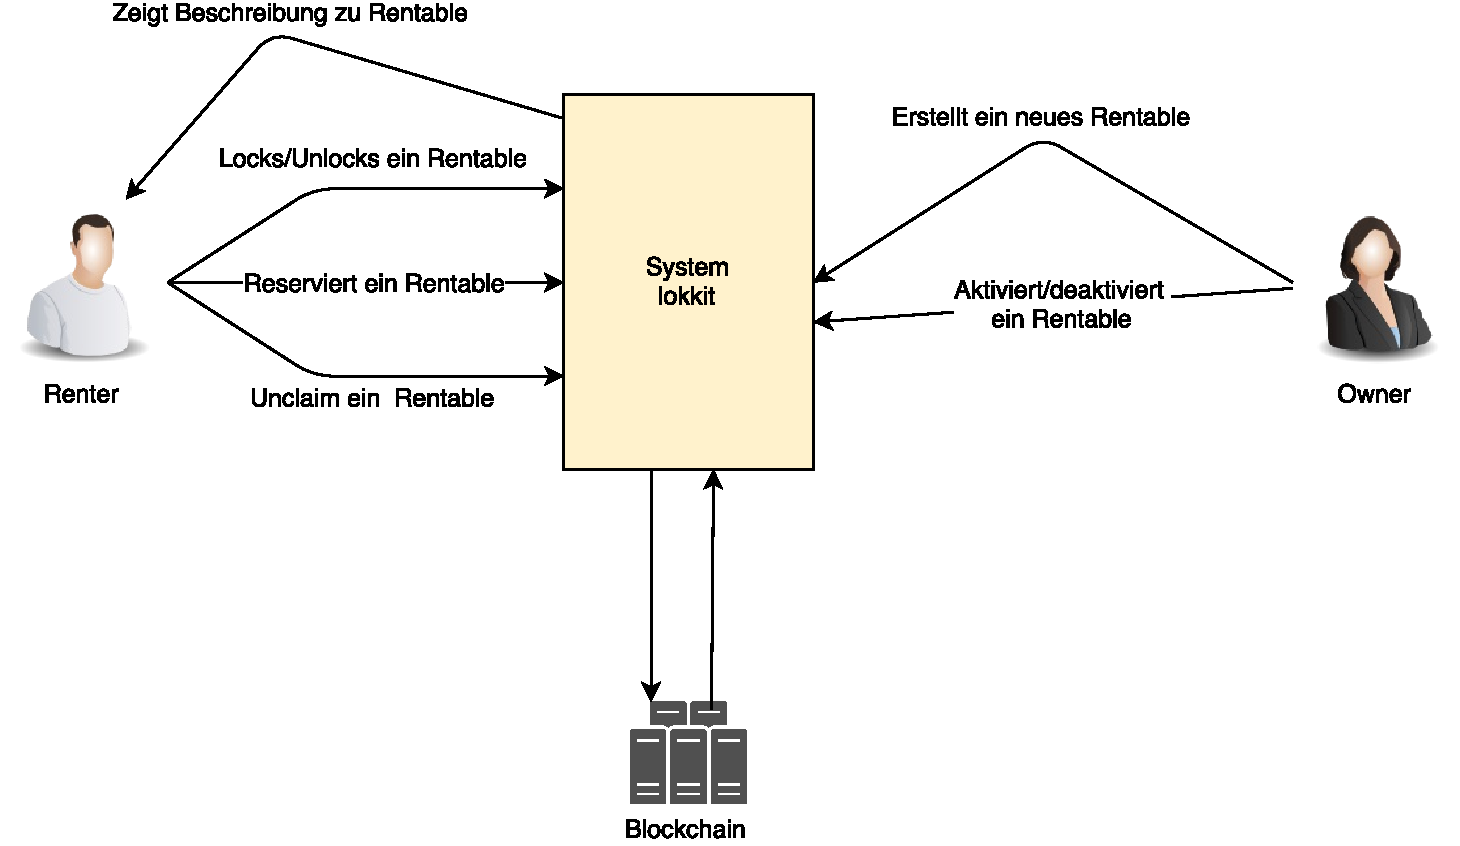
\includegraphics[width=.95\textwidth]{Kontext_Diagram}
\caption{Kontextdiagramm}
\label{fig:Kontextdiagramm}
\end{figure}

\subsection{Systemübersicht IoT}
\label{subsec:Setup_IoT}
Folgend wird das Setup der im Demonstrator zur Verfügung stehender Hardware aufgezeigt.
Übersicht: Raspis, Schliessfächer etc...
\begin{figure}
\centering
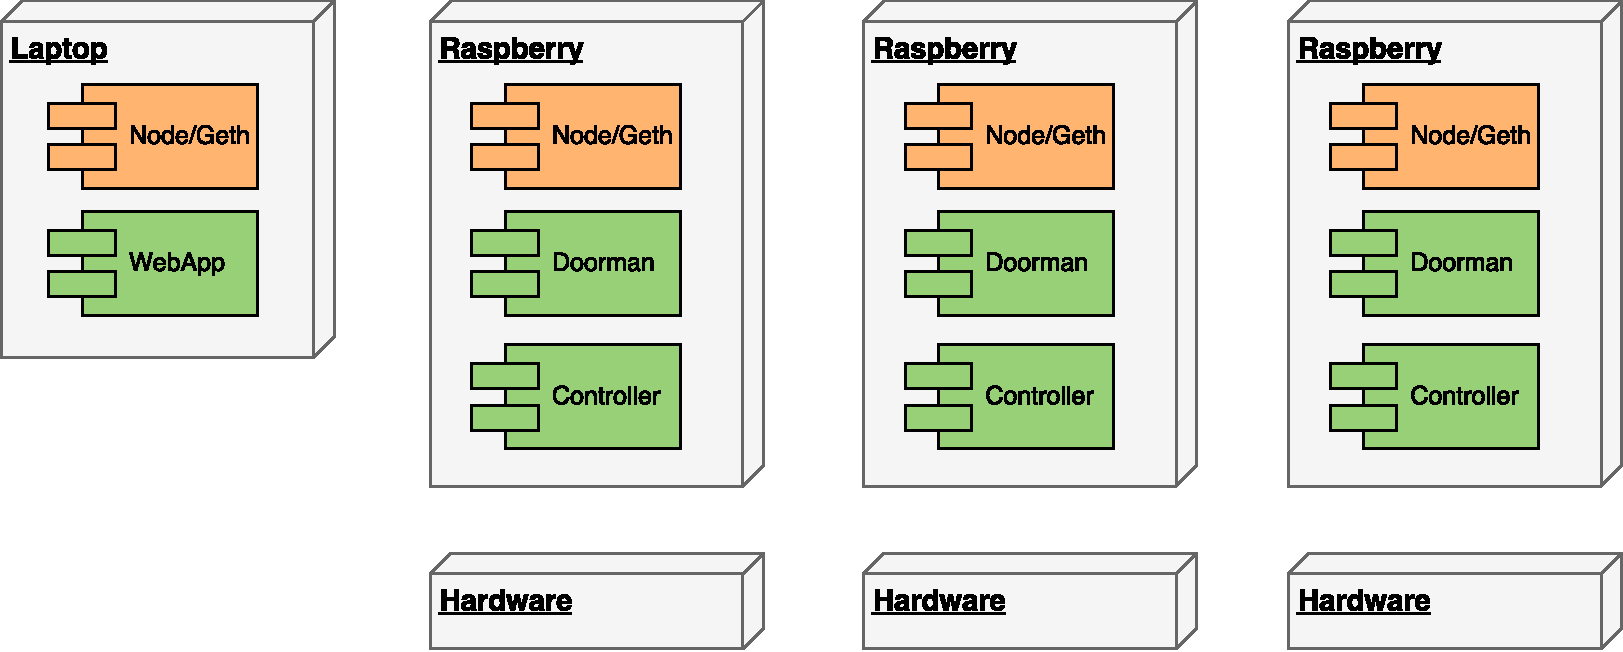
\includegraphics[width=.95\textwidth]{Aufbau_Komponenten}
\caption{Verteilung der Komponenten auf den IoT Geräten}
\label{fig:Aufbau Komponenten}
\end{figure}

\begin{figure}
\centering
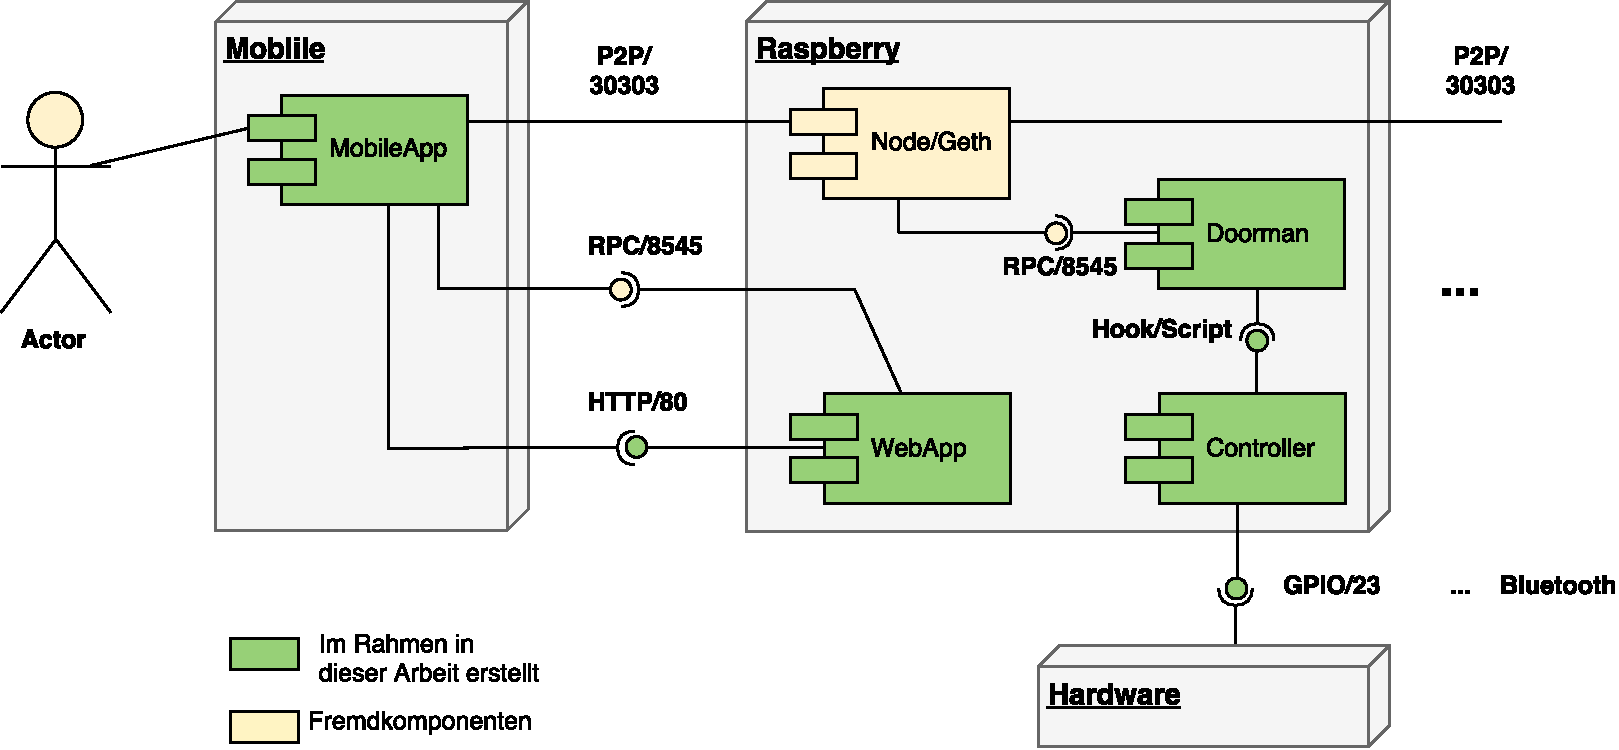
\includegraphics[width=.95\textwidth]{Aufbau_Komponenten_Interface}
\caption{Komponenten und Schnittstellen}
\label{fig:Komponenten und Schnittstellen}
\end{figure}




\section{Komponenten}
\label{sys_sec:Komponenten}
Folgend werden alle im Lokkit System vorhandenen Komponenten, deren Abhängigkeiten und vorgenommene Konfiguration erklärt.

\subsection{Geth}
\label{sys_subsec:Geth}
Geth ist die Referenzimplementation des Ethereum Protokoll. Sie wurde als Node für die Raspberry PIs verwendet.\cite{go-ethereum}

\subsubsection{Konfiguration}
Damit die vom Doorman oder Webapp benötigten Einstellungen in Geth richtig vorgenommen wurden, wird folgend das benutzte Kommando zum Starten von Geth gelistet und einzelne Teile davon erklärt.
\begin{lstlisting}[language=bash,caption={Beispielkommando für das Starten einer Node für Doorman oder Webapp}]
geth --datadir data --nodekeyhex 091bd6067cb4612df85d9c1ff85cc47f259ced4d4cd99816b14f35650f59c322 --rpc --rpcport 8545 --rpcaddr "127.0.0.1" -shh --rpcapi "ws,eth,net,web3,admin,personal,shh" --networkid 42 --ipcpath lokkit  --port "30303" --lightserv 50 --rpccorsdomain "*"
\end{lstlisting}

\begin{table}[H]
\centering
\caption{Kommandozeilenbefehle für Geth\cite[Wiki/Management APIs]{go-ethereum}}
\label{tbl:geth cli}
\begin{tabular}{@{}L{4cm}L{10cm}@{}}
\toprule
geth & Die ausführbare Datei \\ \midrule
--datadir data & der Pfad für alle Daten \\ \midrule
--nodekeyhex X & Wenn die Node las bootnode verwendet wird, muss ein beliebiger nodekeyhex angegeben werden \\ \midrule
--bootnodes X & X ist die enode der bootnode, die zur Entdeckung weiterer Nodes angefragt werden soll \\ \midrule
--rpc & jsonrpc Schnittstelle aktivieren \\ \midrule
--rpcport 8545 & Port für die rpcjson Schnittstelle \\ \midrule
--rpcaddr "127.0.0.1" & Adresse für die jsonrpc Schnittstelle \\ \midrule
-shh & Whisper Nachrichten werden von dieser Node empfangen und weitergeleitet \\ \midrule
--rpcapi "ws,eth,net,web3, admin,personal,shh" & Die möglichen APIs, die über die jsonrpc Schnittstelle zur Verfügung gestellt werden \\ \midrule
--networkid 42 & Dient dazu, gleiche Nodes zu finden \\ \midrule
--ipcpath lokkit & Der Name des IPC Sockets, um die Verbindung von Geth als JavaScript cli zu starten (vgl. \emph{geth attach}) \\ \midrule
--port "30303" & port, der für das Ethereum Protokoll verwendet wird \\ \midrule
--lightserv 50 & Prozent der Rechenleistung, die für light nodes aufgewendet werden darf \\ \midrule
--rpccorsdomain "*" & CORS requests die erlaubt werden sollen. Wichtig für die Verwendung der Webapp. \\ \midrule
 \\ \bottomrule
\end{tabular}
\end{table}

\subsection{Smart Contracts}
Die Datenhaltung und Businesslogik des Lokkit Systems liegt auf der Blockchain in Form von Smart Contracts.
\subsubsection{Rentable}
\label{sys_subsubsec:Rentable}
Eine Instanz dieses Contracts spiegelt ein mietbares Objekt wieder. Nachfolgend werden Einzelheiten zur Implementation und Verwendung aufgeführt.

\paragraph{Attribute}
\label{sys_para:Rentable_Attribute}
Attribute eines Rentable können gelesen und gesetzt werden. Lesen wird durch die automatische Lesefunktion von Solidity gemacht, gesetzt werden die Attribute durch eine entsprechende Funktion, die den prefix \emph{set} hat und den neuen Wert als einzigen Parameter annimmt. Wichtig zu beachten ist, dass die Funktion zum Ändern des Owners nicht setOwner sondern \emph{transferOwnership} heisst. Dieser Name widerspiegelt die Tatsache, dass der Besitz übertragen wird und sollte nicht leichtfertig mit einer \emph{set} Funktion verwechselt werden. Wenn eine Eigenschaft mittels einer \emph{set} Funktion verändert wird, wird das OnUpdate\emph{X} Event ausgelöst, wobei X für die veränderte Eigenschaft steht. 

\begin{longtable}{@{}llL{9cm}@{}}
\caption{Rentable Eigenschaften}\label{tbl:Rentable_Eigenschaften}\\
\toprule
Name & Typ & Beschreibung \\ \midrule
owner & address   & Besitzer des Rentable Objektes. Kann Eigenschaften verändern und privilegierte Funktionen ausführen.\\
description & string   & Beschreibung des Rentable Objektes.\\
location & string   & Standort des Rentables.\\
costPerSecond & uint   & Kosten des Rentables in Wei\footnote{$1 Ether = 10^{18}
Wei$} pro Sekunde.\\
deposit & uint & Menge Wei, die hinterlegt werden muss. Wird zurückerstattet, wenn \emph{unclaim} oder \emph{forceUnclaim} aufgerufen werden (vgl. \ref{sys_para:claim_unclaim}).\\
\end{longtable}

\paragraph{Berechnung der Kosten}

\paragraph{unclaim und forceUnclaim}
\label{sys_para:claim_unclaim}
Um die regelkonforme Rückgabe eines Rentables festzustellen, muss vom Mieter die Funktion \emph{unclaim} aufgerufen werden (vgl. \ref{tbl:Rentable_Funktionsuebersicht}). Damit bestätigt der Mieter, dass das Rentable nicht länger verwendet wird. Sollte der Mieter nicht unclaim aufrufen, kann der \emph{owner} zu einem Zeitpunkt nach der Reservation die Funktion \emph{forceUnclaim} aufrufen (vgl. \ref{tbl:Rentable_Funktionsuebersicht}), um das Depot seinen \emph{pendingRefunds} gutzuschreiben.

\paragraph{pendingRefunds}
\label{sys_para:pendingRefunds}
Falls zu viel Ether an den Contract überwiesen wird oder eine Rückerstattung des \emph{deposit} erwirkt wurde, werden die Beträge in die \emph{pendungRefunds} des Rentables eingetragen. Auch der die Gutschriften, die der Owner bekommt werden in dieser Form gespeichert. Die \emph{pendingRefunds} können explizit aus dem Smart Contract abgehoben werden.\cite[Miscellaneous/Introduction to Smart Contracts]{solidity.readthedocs.io}

\paragraph{Funktionsübersicht}

L: Lesefunktion, S: Schreibfunktion, C: Konstruktor, E: Event

Alle Funktionen, die einen Zeitpunkt als Parameter (\emph{start} oder \emph{end}) annehmen, erwarten diesen im Unix Epoch Format.

\begin{longtable}{@{}lcL{9cm}@{}}
\caption{Rentable Funktionen und Events}\label{tbl:Rentable_Funktionsuebersicht}\\
\toprule
Name & Typ & Beschreibung \\ \midrule
allReservations     & L   & Gibt alle Reservationen als Array zurück. Eine Reservation besteht aus einem Array mit drei Einträgen: Startzeit, Endzeit, Ob die aufrufende Adresse der Mieter ist.\\
 & & Parameter: keine \\\midrule
reservedAt          & L   & Gibt zurück, ob das Rentable am gegebenen Zeitpunkt \emph{time} reserviert ist.\\ & & Parameter: \emph{time} \\\midrule
reservedBetween     & L   & Gibt zurück, ob das Rentable zwischen den gegebenen Zeitpunkten \emph{start} und \emph{end} reserviert ist.\\ & & Parameter: \emph{start}, \emph{end} \\\midrule
currentRenter       & L   & Gibt die Adresse des momentanen Mieters zurück. Wenn das Rentable momentan nicht vermietet ist, wird 0 zurückgegeben.\\ & & Parameter: keine \\\midrule
costInWei           & L   & Gibt die Kosten in Wei für die Zeit zwischen \emph{start} und \emph{end} zurück.\\ & & Parameter: \emph{start}, \emph{end} \\\midrule
myPendingRefund     & L   & Gibt zurück, wie viel Ether die aufrufende Adresse noch abheben kann.\\ & & Parameter: keine \\ \midrule
currentReservation  & L   & Gibt die momentane Reservation zurück als Array mit drei Einträgen: Startzeit, Endzeit, Ob die aufrufende Adresse der Mieter ist.\\ & & Parameter: keine \\\midrule
transferOwnership   & S   & Setzt den \emph{owner} des Rentables auf die angegebene Adresse \emph{newOwner}.\\ & & Parameter: \emph{newOwner} \\\midrule
setDescription   & S   & Setzt \emph{description} des Rentables auf den angegebenen Text \emph{newDescription}.\\ & & Parameter: \emph{newDescription} \\\midrule
setLocation   & S   & Setzt die \emph{location} des Rentables auf den angegebenen Text \emph{newLocation}.\\ & & Parameter: \emph{newLocation} \\\midrule
setCostPerSecond   & S   & Setzt die \emph{costPerSecond} des Rentables auf die angegebene Menge \emph{newCostPerSecond}.\\ & & Parameter: \emph{newCostPerSecond} \\\midrule
setDeposit   & S   & Setzt das \emph{peposit} des Rentables auf die angegebene Menge \emph{newDeposit}.\\ & & Parameter: \emph{newDeposit} \\\midrule
rent                & S   & Mietet das Rentable zwischen \emph{start} und \emph{end} für die sendende Adresse.\newline{}Vorbedingungen: start muss früher als end sein. Die Menge Ether muss für die Reservation ausreichen (vgl. \emph{costInWei}). \\ & & Parameter: \emph{start}, \emph{end} \\\midrule
unclaim         & S   & Retourniert ein Rentable während die gemietete Zeit noch nicht abgelaufen ist. Der bezahlte Betrag für die zusätzliche Zeit wird gleichmässig zwischen \emph{renter} und \emph{owner} aufgeteilt. Das \emph{deposit} wird dem refund des \emph{renter}s gutgeschrieben.\\ & & Parameter: keine \\\midrule
forceUnclaim         & S   & Retourniert alle Reservations, die in der Vergangenheit liegen und auf welchen nicht unclaim aufgerufen wurde. Das \emph{deposit} wird dem refund des \emph{owner}s gutgeschrieben.\\ & & Parameter: keine \\\midrule
withdrawRefunds     & S   & Hebt alle bestehenden Rückerstattungen einer Adresse vom Rentable ab und überweist sie auf das Konto der sendenden Adresse\\ & & Parameter: keine \\\midrule
Rentable            & C   & Erstellt ein neues Rentable mit den angegebenen Parametern und der sendenden Adresse als \emph{owner}.\\ & & Parameter: \emph{pdescription}, \emph{plocation}, \emph{pcostPerSecond}, \emph{pdeposit} \\ \midrule
OnRent              & E   & Wird ausgelöst, wenn versucht wird, das Rentable zu mieten (vgl. Funktion \emph{rent}). \emph{success} gibt an, ob die Reservation erfolgreich war. \emph{msg} beinhaltet eine Statusmeldung zum Funktionsaufruf (Fehlerbeschreibung im Fehlerfall).\\ & & Parameter: \emph{success}, \emph{renter}, \emph{start}, \emph{end}, \emph{msg} \\ \midrule
OnTransferOwnership              & E   & Wird ausgelöst, wenn \emph{owner} durch die \emph{transferOwnership} Funktion verändert wird.\\ & & Parameter: \emph{oldOwner}, \emph{newOwner} \\ \midrule
OnUpdateDescription              & E   & Wird ausgelöst, wenn \emph{description} durch die \emph{setDescription} Funktion verändert wird.\\ & & Parameter: \emph{oldDescription}, \emph{newDescription} \\ \midrule
OnUpdateLocation              & E   & Wird ausgelöst, wenn \emph{location} durch die \emph{setLocation} Funktion verändert wird.\\ & & Parameter: \emph{oldLocation}, \emph{newLocation} \\ \midrule
OnUpdateCostPerSecond              & E   & Wird ausgelöst, wenn \emph{costPerSecond} durch die \emph{setCostPerSecond} Funktion verändert wird.\\ & & Parameter: \emph{oldCostPerSecond}, \emph{newCostPerSecond} \\ \midrule
OnUpdateDeposit              & E   & Wird ausgelöst, wenn \emph{deposit} durch die \emph{setDeposit} Funktion verändert wird.\\ & & Parameter: \emph{oldDeposit}, \emph{newDeposit} \\
\bottomrule
\end{longtable}

\subsection{Webapp}
\label{sys_subsec:Webapp}

Die Webapp für Lokkit stellt eine Gerätunabhängige Benutzeroberfläche für die Interaktion mit dem Lokkit System zur Verfügung. Es wird mindestens ein Account, mit genügend Ether, vorausgesetzt, um mit den Rentable Objekten interagieren zu können.

\begin{figure}[H]
\centering
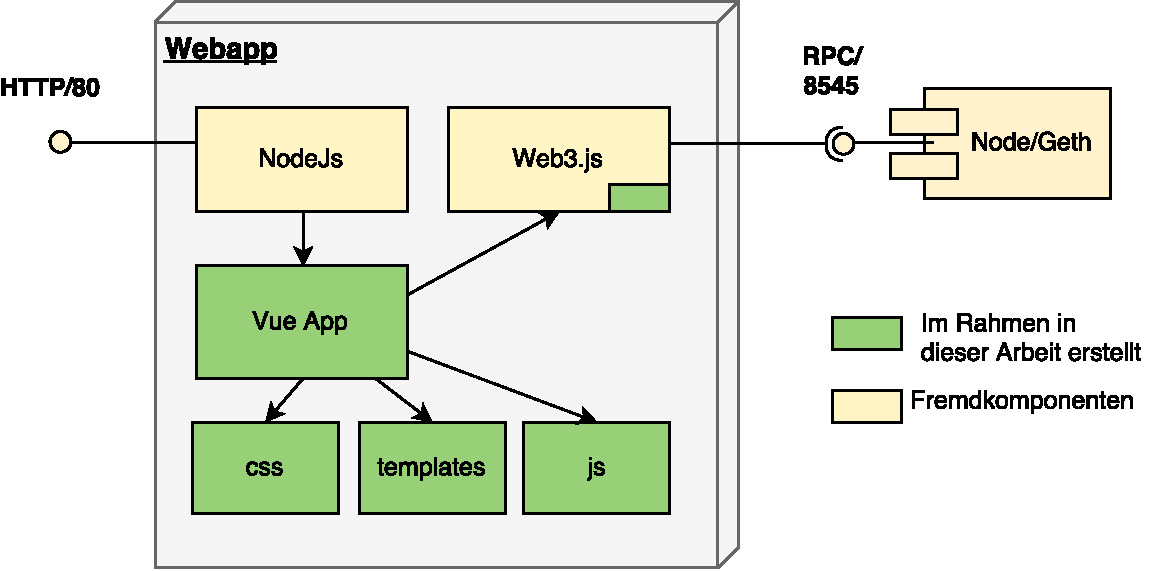
\includegraphics[width=.75\textwidth]{Aufbau_Webapp}
\caption{Interner Aufbau der Webapp}
\label{fig:Aufbau der Webapp}
\end{figure}

\paragraph{}
Die Webapp ist eine Single Page Aplication (SPA), basiert auf NodeJS und benutzt VueJS\footnote{\url{https://vuejs.org/}} mit Material Design für die Benutzeroberfläche. Um mit der Blockchain zu interagieren wird die Web3.js Library verwendet, welche die \emph{RPC/8545} Schnittstelle des Geth Nodes implementiert. 
Die Schnittstelle gegen Aussen ist \emph{HTTP/80}. Diese ist ungeschützt und wird bei der Installation der Webapp durch einen Webserver geschützt. Die Abbildung \ref{fig:Aufbau der Webapp} zeigt eine grobe Übersicht über die verschiedenen Elemente.


\subsubsection{Webapp Abhängikeiten}
Nachfolgend ist die Liste aller zur Laufzeit benötigten Module und Libraries.

\begin{table}[H]
\centering
\caption{Webapp Runtime Abhängigkeiten}
\label{tbl:Webapp Runtime Abhängigkeiten}
\begin{tabular}{@{}lll@{}}
\toprule
Library/Modul         & Version & Beschreibung
\\ \midrule
material-design-icons & 3.0.1 & Offizielle Icons für Material Design                       \\
mdi                   & 1.9.33 & Community Icons für Material Design                       \\
moment                & 2.18.1 & Javascript Datum und Zeit Library                         \\
qrcode-reader         & 1.0.0  & Library zum Dekodieren von QR-Codes                       \\
vue                   & 2.2.2  & Vue.js                                                    \\
vue-material          & 0.7.1  & Material Design Komponenten für Vue.js                    \\
vue-resource          & 1.3.1  & Resource Management für Vue.js                            \\
vue-router            & 2.3.0  & Routing für Vue.js                                        \\
vue-toasted           & 1.0.27 & Zum Anzeigen von Status- und Fehlermeldungen              \\
vuex                  & 2.3.1  & Zentralisiertes State Management für Vue.js               \\
vuex-localstorage     & 1.0.0  & Zur Speicherung der Session im Local Storage des Browsers \\
web3                  & web.js & Library für die Kommunikation in die Blockchain           \\ 
\bottomrule
\end{tabular}
\end{table}


\subsubsection{Webapp Projektstruktur}
Die Projektstruktur ist durch die Verwendung von \emph{NPM} gegeben. Nachfolgend wird kurz eine Übersicht über die Verzeichnisse gegeben.

\begin{minipage}{\textwidth}
\begin{lstlisting}[style=tree,caption={Projektstruktur der Webapp}]
webapp
├── build                   # Build Verzeichnis
├── certs                   # Zertifikate
│   ├── server.crt
│   └── server.key
├── config                  # Konfiguration für dev/prod/test
├── debian                  # Konfiguration für das Debian Paket
├── index.html              # Hauptseite
├── node_modules            
├── package.json            # Definiert Build Process und Abhängigkeiten
├── README.md               
├── src                     # Sourcen
│   ├── App.vue
│   ├── components          # Enthält all Komponenten, Views, etc.
│   ├── main.js
│   ├── router              # Definiert das Routing
│   ├── services            # Enthält Web3 Abstraktionsservice
│   └── store.js            
├── static
│   ├── lokkit_icon_100.png
│   └── lokkit_icon_400.png
├── test                     
│   ├── e2e
│   └── unit
└── web3.js                 # Gepatchtes Web3.js
\end{lstlisting}
\end{minipage}

\subsubsection{Ethereum Node}
Die Vorbedingung zur Verwendung der Webapp ist eine laufende und korrekt konfigurierte Ethereum Node, die die jsonrpc Schnittstellen \emph{eth}, \emph{shh}, \emph{personal} auf dem Port 8545 zur Verfügung stellt.


\subsubsection{Webapp Funktionalität und Design}
Die Oberfläche kann grundsätzlich in vier verschiedene Ansichten unterteilt werden. Die erste Ansicht zeigt das Menu zur Navigation zwischen den Ansichten (vgl. Abbildung \ref{fig:4 Ansichten der Webapp} (a)). Das Menu bietet neben dem Absprung auf andere Ansichten auch die Möglickeit den Account zu wechseln. Weiter kann der \emph{Local Storage} gelöscht werden, wodurch alle bereits eingescannten Rentables wieder verschwienden. Die Abbildung \ref{fig:4 Ansichten der Webapp} (b) stellt die drei bereits eingescannten Rentables in Form von einer Liste dar. 
Ebenfalls bietet die Webapp die Möglickeit an sich mit einem beliebigen Node zu verbinden. Diese Einstellung ist z.B. in der Netzwerkansicht (vgl. Abbildung \ref{fig:4 Ansichten der Webapp} (c)) untergebracht. Für jedes Rentable gibt es ausserdem eine Detailansicht, welche die Interaktion mit dem Smart Contract in der Blockchain darstellt. Über diese Ansicht, kann der Benutzer das Rentable reservieren, schliessen, öffnen und wieder zurück geben. Die Abbildung \ref{fig:4 Ansichten der Webapp} (d) präsentiert die Detailansicht.

\paragraph{QrCode Leser}
\label{sys_para:QrCode Leser}
Die Webapp benötigt für das Dekodieren des QrCode Zugriff auf eine Kamera. Dieses Feature basiert rein auf dem HTML5 Standard. Es sind keine Browserplugins nötig. Dekodiert wird mit der Library ``qrcode-reader''. Der Ablauf ist wie folgt:

\begin{enumerate}
    \item Die Webseite öffnet einen Live-Stream der Webcam
    \item Eine Javascript-Funktion zeichnet im Sekundentakt ein Bild auf ein Canvas (HTML Element)
    \item Anschliessend kann die qrcode-reader Library das Bild im Canvas dekodieren
\end{enumerate}

Der QrCode muss eine gültige Rentable Adresse (z.B. 0xde93b2965af6a49161f597604c600af9ea07883a) enthalten. Ist dies nicht der Fall, wird eine Fehlermeldung angezeigt.


\begin{figure}[H]
\centering\small
\setlength{\tabcolsep}{0mm}	% alle Spaltenränder auf 0mm
\begin{tabular}{c@{\hspace{12mm}}c} % mittlerer Abstand = 12mm
  \frame{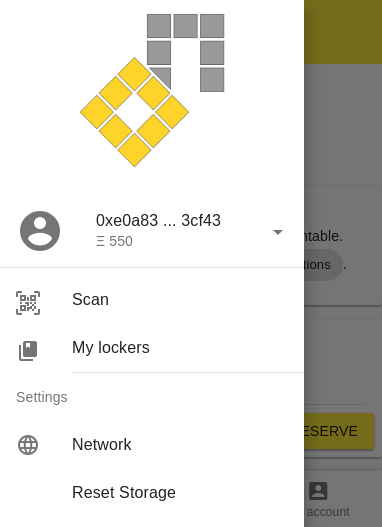
\includegraphics[width=.45\textwidth]{webapp_menu}} &
  \frame{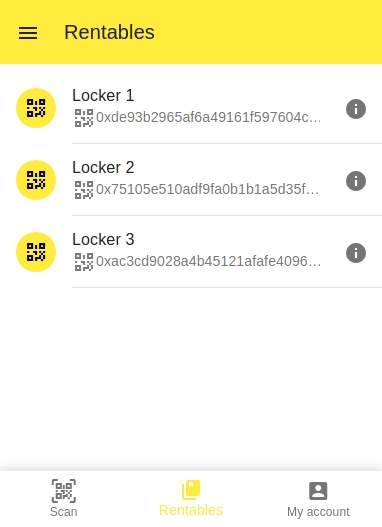
\includegraphics[width=.45\textwidth]{webapp_rentables}} \\
  (a) & (b)
  \\[.5cm]	%vertical extra spacing (4 points)
  \frame{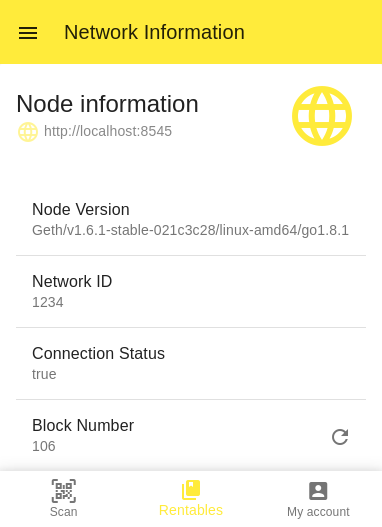
\includegraphics[width=.45\textwidth]{webapp_network}} &
  \frame{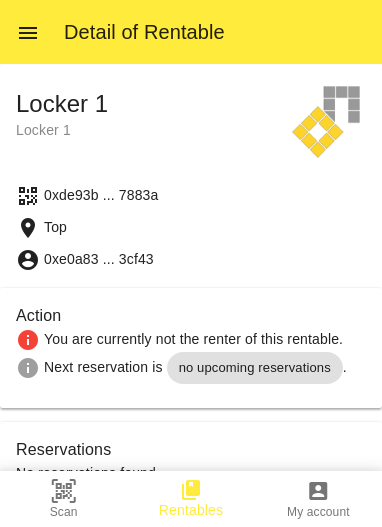
\includegraphics[width=.45\textwidth]{webapp_rentable1}} \\
  (c) & (d)
\end{tabular}
%
\caption{Webapp 4 Ansichten der Webapp-- 
Menu (a), Liste aller gescannten Rentables (b),
Netzwerkinformationen (c), Details eines Rentables (d).}
\label{fig:4 Ansichten der Webapp}
\end{figure}


\subsection{Android App}
\label{sys_subsec:Android_App}
Die Android App startet und administriert eine Ethereum Node mit dem Lokkit Genesis Block, um die Verwendung vom Lokkit Webapp (vgl. \ref{sys_subsec:Webapp}) auf einem Androidgerät zu ermöglichen.

\subsubsection{Architektur}
Die Android App besteht aus einer Activity zur Benutzerinteraktion und aus einem Service, der an die Activity gebunden wird. Durch die Verwendung eines Service kann die Ethereum Node im Hintergrund weiter laufen, auch wenn die Activity minimiert wurde. Die Node selbst wird von der Statusgo (vgl. \ref{sys_subsubsec:Statusgo}) Library erstellt und ausgeführt. Die Webapp (vgl. \ref{sys_subsec:Webapp}) greift dabei auf die RPC Schnittstelle auf Port 8545 zu, um mit der lokalen Node zu interagieren.

\begin{figure}[H]
\centering\small
  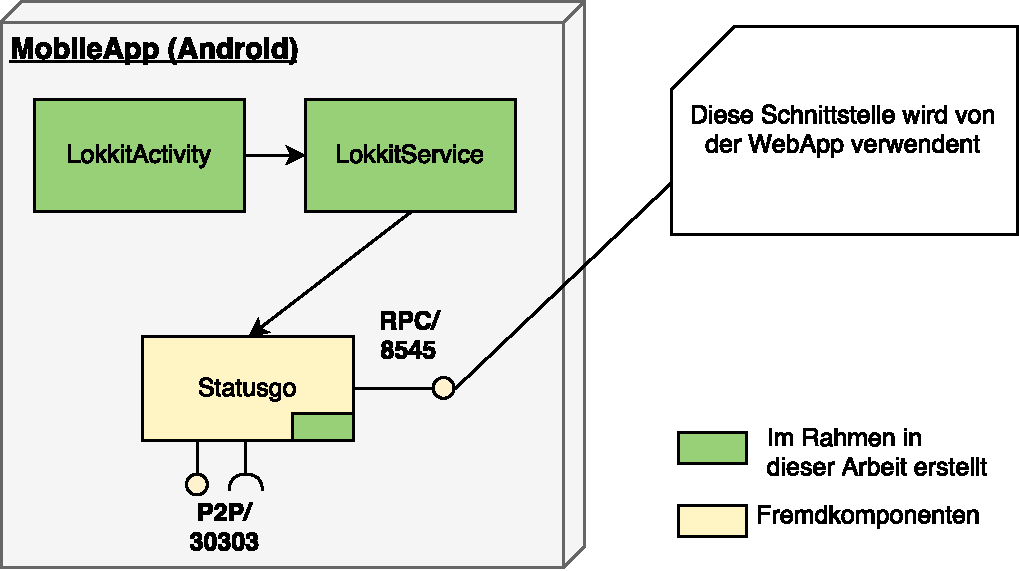
\includegraphics[width=.75\textwidth]{Aufbau_AndroidApp}
\caption{Interner Aufbau der AndroidApp}
\label{fig:Aufbau_AndroidApp}
\end{figure}

\subsubsection{Ablauf}
Wenn die Android App das erste mal gestartet wird, wird der Lokkit Service gebunden und die Activity nach einem Passwort für den Account gefragt (vgl. \ref{fig:android_sequence_start}). Bei nachfolgenden Starts wird der erstellte Account geladen und die Activity nach dessen Password gefragt. Wenn die Verbindung erfolgreich hergestellt werden konnte, wird das Webapp geladen.

\begin{figure}[H]
\centering\small
\setlength{\tabcolsep}{0mm}	% alle Spaltenränder auf 0mm
\begin{tabular}{c@{\hspace{12mm}}c} % mittlerer Abstand = 12mm
  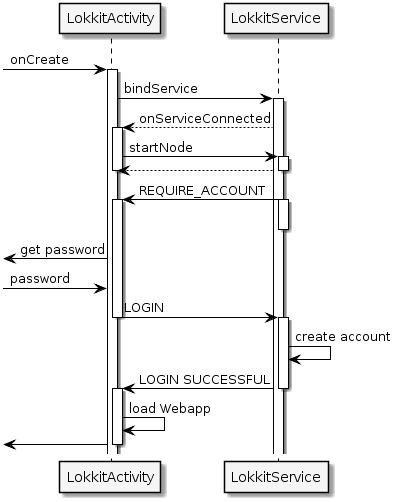
\includegraphics[width=.48\textwidth]{android_sequence_start_new} &
  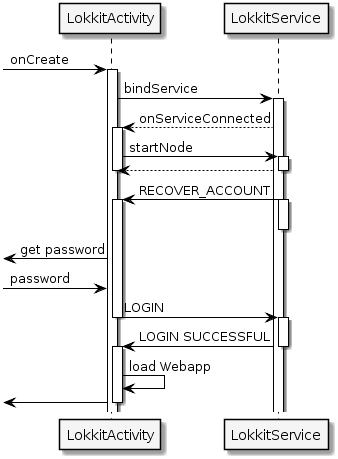
\includegraphics[width=.42\textwidth]{android_sequence_start_existing} \\
  (a) & (b)
\end{tabular}
%
\caption{erster Start (a), spätere Starts (b)}
\label{fig:android_sequence_start}
\end{figure}

\subsubsection{Statusgo}
\label{sys_subsubsec:Statusgo}
Diese Subkomponente implementiert das Ethereum Protokoll und weitere Funktionalität von status-im. Die API kann über die statische Klasse \emph{Statusgo}\footnote{Im Paket com.github.status\_im.status\_go.cmd zu finden} in Java verwendet werden. Diese Library implementiert das gesamte Ethereum Protokoll und ermöglicht das starten einer Ethereum Node als Light Node (vgl. \ref{para:Light_Node}).\cite[wiki/Build-Process-Explained]{github.com/status-im/status-go}

\subsubsection{Lokkit Service}
Der Lokkit Service konsumiert das statusgo-android Modul. Der Service wird bei Start der Applikation gestartet und bei Beenden der Applikation gestoppt. Der Service sendet und empfängt Intents (vgl. \ref{tbl:LokktService_SendIntents}, \ref{tbl:LokktService_ListenIntents}) für die Interaktion mit der Lokkit Activity (vgl. \ref{sys_subsubsec:Lokkit_Activity}).\cite[Bound Services]{developer.android.com}

Die Statusgo Library bedingt, dass eine erstellte Transaktion zuerst durch Statusgo freigegeben wird, bevor sie in die \emph{pending transactions} von geth aufgenommen wird (vgl. \ref{sys_subsec:Geth}). Dabei weist Statusgo jeder Transaktion eine id zu. Diese id ist spezifisch für Statusgo und hat keine Bedeutung im Ethereum Protokoll.

\begin{table}[H]
\centering
\caption{Intents, die vom Lokkit Service gesendet werden}
\label{tbl:LokktService_SendIntents}
\begin{tabular}{@{}L{3cm}L{2cm}L{10cm}@{}}
\toprule
action & extras & Beschreibung \\ \midrule
io.lokkit.\newline{}TRANSACTION\newline{}\_QUEUED\newline{} & id, from, to, value, gas, gasPrice & Wird versendet, wenn eine neue Transaktion von Statusgo erhalten wurde. Diese muss mit io.lokkit.COMPLETE\_TRANSACTION oder io.lokkit.DISCARD\_TRANSACTION bestätigt werden. \\\midrule
io.lokkit.\newline{}COMPLETE\newline{}\_TRANSACTION\newline{}\_FAILED & id, reason & Wird als Antwort auf io.lokkit.COMPLETE\_TRANSACTION gesendet, wenn eine Transaktion nicht bestätigt werden konnte. \\\midrule
io.lokkit.\newline{}COMPLETE\newline{}\_TRANSACTION\newline{}\_SUCCESSFUL & id & Wird als Antwort auf io.lokkit.COMPLETE\_TRANSACTION gesendet, wenn eine Transaktion erfolgreich bestätigt werden konnte. \\\midrule
io.lokkit.\newline{}LOGIN\newline{}\_SUCCESSFUL & - & Wird als Antwort auf io.lokkit.LOGIN gesendet, wenn das in io.lokkit.LOGIN gesendete Password für das Entsperren des gespeicherten Accounts verwendet werden konnte. \\\midrule
io.lokkit.\newline{}RECOVER\newline{}\_ACCOUNT & address, mnemonic & Wird gesendet, wenn der Service beim Start einen Account findet. Muss mit io.lokkit.LOGIN beantwortet werden. \\\midrule
io.lokkit.\newline{}REQUIRE\newline{}\_ACCOUNT & - & Wird gesendet, wenn ein Account gefunden wurde. Muss mit io.lokkit.LOGIN beantwortet werden. \\\midrule
io.lokkit.\newline{}COMPLETE\newline{}\_TRANSACTION & id & Da der Demonstrator nur die Lokkit webapp bedient, wurde der Einfachheit halber diese Funktionalität umgangen, indem der Service die Nachfrage nach de Account sich selbst beantwortet. \\
\bottomrule
\end{tabular}
\end{table}

\begin{table}[H]
\centering
\caption{Intents, die vom Lokkit Service verarbeitet werden}
\label{tbl:LokktService_ListenIntents}
\begin{tabular}{@{}L{3cm}L{2cm}L{10cm}@{}}
\toprule
action & extras & Beschreibung\\ \midrule
io.lokkit.\newline{}COMPLETE\newline{}\_TRANSACTION & id, password & Bestätigt die Transaktion mit id id durch Verwendung des momentanen Accounts (vgl. Statusgo.Login()) und des angegebenen Passworts. Die Transaktion wird erst durch Senden dieses Intents in die Liste der pending transactions aufgenommen. Aufruf wird bestätigt durch einen Intent mit action io.lokkit.COMPLETE\_TRANSACTION\_SUCCESSFUL, falls erfolgreich oder io.lokkit.COMPLETE\_TRANSACTION\_FAILED falls nicht erfolgreich. \\\midrule
io.lokkit.\newline{}DISCARD\newline{}\_TRANSACTION  & id           & Verneint die Transaktion mit id id. Diese Funktionalität kann verhindern, dass ohne Erlaubnis des Benutzers eine Transaktion von einer DAPP ausgelöst wird. Aufruf wird nicht bestätigt.\\\midrule
io.lokkit.\newline{}LOGIN & password     & Meldet den persistierten Benutzer an. Aufruf wird bestätigt durch einen Intent mit action io.lokkit.LOGIN\_SUCCESSFUL, falls erfolgreich oder io.lokkit.RECOVER\_ACCOUNT falls nicht erfolgreich.
\\ \bottomrule
\end{tabular}
\end{table}

\subsubsection{Lokkit Activity}
\label{sys_subsubsec:Lokkit_Activity}
Wenn die Lokkit App gestartet wird, wird die Lokkit Activity geöffnet. Diese Activity dient dazu, die Interaktion des Benutzers mit dem Lokkit Service sicherzustellen. Falls der Lokkit Service Eingaben benötigt, wird die Activity benachrichtig und wird dementsprechend den Benutzer nach der Eingabe fragen, bspw. wenn ein Passwort für einen neuen Account angegeben werden muss (vgl. \ref{fig:sys_android_new_account}).

\begin{figure}[H]
\centering
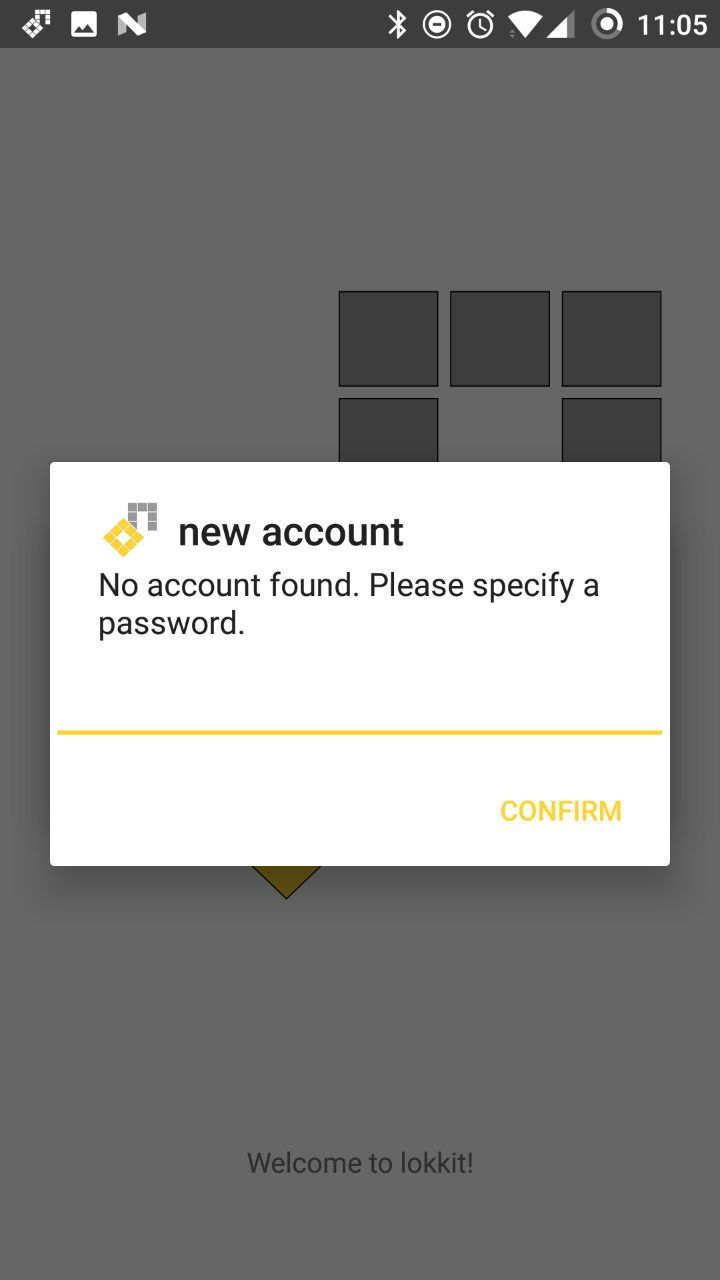
\includegraphics[width=.40\textwidth]{android_new_account}
\caption{Beispielansicht: Activity fragt den Benutzer nach einem Passwort für einen neuen Account}
\label{fig:sys_android_new_account}
\end{figure}



\subsection{Doorman}
\label{sys_subsec:Doorman}
Doorman verbindet auf eine Ethereum Node, die die shh und eth Protokolle aktiviert hat und hört auf Whisper v5 Nachrichten für die in der Konfiguration definierten Rentables. Wenn die payload der Nachrichten der Definition in der Real-Time Kommunikationsschnitstelle (vgl. \ref{sys_subsec:Real_Time_Kommunikationsschnittstelle}) entsprechen und der Absender validiert werden konnte, wird ein Script ausgeführt, das als Parameter die Adresse des Rentables, sowie das command (vgl. \ref{sys_subpara:Command}) erhält.

\subsubsection{Konfiguration}
\label{sys_subsec:Doorman_Konfiguration}
Die Konfiguration des Doorman wird aus einer yml Datei\footnote{\url{https://fdik.org/yml/}} gelesen. Die Datei besitzt einen root mit Namen \emph{doorman} und Attribute für die Ethereum Node, verwendete Rentable Smart Contract Adressen und auszuführendes Script bei Erhalt einer validen Nachricht.
\begin{lstlisting}[language=yml,caption={Beispielkonfiguration für Doorman}]
doorman:
    node_ip: 127.0.0.1
    node_rpc_port: 8545
    rentable_addresses:
        - "0xf16801293f34fc16470729f4ac91185595aa6e10"
        - "0x298345dddd494c51061da2ae137df3129ce14b69"
    script: open_close_device.bat
\end{lstlisting}

\paragraph{node\_ip}
Die Url der Ethereum Node, zu der eine Verbindung aufgebaut werden soll. Diese Node muss das shh Protokoll und auch die shh API aktiviert haben (vgl. \ref{para:Whisper}). Die Adresse ist als IP anzugeben. Informationen zum Protokoll wie \emph{http://} sind auszulassen.
\paragraph{node\_rpc\_port}
Der Port, auf dem Doorman zu der Ethereum Node verbinden soll. Der Standardport ist 8545.
\paragraph{rentable\_address}
Die Adressen der Smart Contracts vom typ Rentable (vgl. \ref{sys_subsubsec:Rentable}), auf deren Nachrichten gehört werden sollen. Wird eine ungültige Rentable Adresse angegeben, werden die Befehle nicht ausgeführt.
\paragraph{script}
Das script, das ausgeführt werden soll.

\section{Interne Schnittstellen}
In diesem Abschnitt werden die internen Schnittstellen des lokkit Systems beschrieben.

\subsection{Real-Time Kommunikationsschnittstelle}
\label{sys_subsec:Real_Time_Kommunikationsschnittstelle}

\subsubsection{Aufbau der Nachricht}
Für das gesamte von Whisper v5 versendete Packet wird der Ausdruck \emph{Envelope} verwendet. Die darin enthaltene textbasierte Nachricht, die einen validen JSON-String beinhaltet, wird als \emph{Payload} bezeichnet. Da Whisper v5 nur textbasierte Payloads unterstützt, wurde eine Nachricht im \acrshort{JSON} Format definiert, die eine strukturierte Möglichkeit zur Datenübermittlung ermöglicht. Diese wird übermittelt, indem sie vom Sender zu einer String-Repräsentation umgewandelt wird und nach Erhalt beim Empfänger wiederum zu einem JSON geparst wird. Das definierte Objekt besitzt zwei Attribute: \emph{digest} (vgl. \ref{sys_para:Digest}), nachfolgend Diges und \emph{message} (vgl. \ref{sys_para:Message}), nachfolgend Message Objekt. 

\begin{lstlisting}[language=json,caption={Beispiel einer lokkit JSON Nachricht}]
{
  digest: \#TODO: insert digest,
  message: {
    command: "open",
    rentableAddress: "0x4cbee4df58c717f47a5e6e8d305a450fcdbe1e24",
    key: \#TODO:INSERT SAMPLE KEY
  }
}
\end{lstlisting}

\paragraph{Message}
\label{sys_para:Message}
Das Message Objekt innerhalb der Payload enthält drei Attribute: \emph{command}, \emph{rentableAddress} und \emph{key}. Funktional relevant für den Empfänger sind dabei nur command und rentableAddress. Das key Attribut ist eine zusätzliche Sicherheit, um Replay-Angriffe mit demselben Packet zu verhindern, bei welchen dasselbe Paket von einem anderen Sender versendet wird.
\subparagraph{Command}
\label{sys_subpara:Command}
Dieses Feld teilt den Befehl mit, den das mietbare Objekt ausführen soll. Abhängig von der jeweiligen Implementation des IoT Geräts kann dieses Feld andere Werte beinhalten. Im Beispiel von lokkit werden \emph{open} und \emph{close} für Schliessfächer geschickt. Weitere Befehle sind denkbar, die ebenfalls den Doorman als Empfänger verwenden.
\subparagraph{Rentable Address}
Damit der Empfänger weiss, welches mietbare Objekt von dem Befehl angesteuert werden soll, wird die gesamte Adresse mitgegeben. Alternativ könnte dieses Feld weggelassen werden und über das Topic der Nachricht bestimmt werden.

Da die 
\\\#TODO:Muss envelope.payload.message.rentableAddress vorhanden sein? Warum nicht nur envelope.topic und Vergleich auf sha3 hashes beim empfangen?

\subparagraph{Key}
\label{sys_para:Key}
Dieses Feld beinhaltet den öffentlichen Schlüssel eines asymmetrischen Schlüsselpaars des Senders. Derselbe Schlüssel muss zum signieren des Envelopes verwendet werden\footnote{Diese Signatur ist optional bei Whisper, wird jedoch für lokkit Envelopes vorgeschrieben}. Der öffentliche Schlüssel des für die Signatur verwendeten Schlüsselpaars wird ebenfalls im Envelope als Feld \emph{sig} mitgeschickt. Bei einer validen Nachricht sind also das Feld \emph{key} des Message Objektes und das Feld \emph{sig} des Envelopes identisch\footnote{Für weitere Informationen für diese Deisgn-Entscheidung, vgl. \ref{para:Replay_Attack} \#TODO: verweis von sysspec zu bericht?}.

\paragraph{Digest}
\label{sys_para:Digest}
Um den Digest eines Message Objekts zu erzeugen wird die Funktion \emph{web3.eth.sign(...)}\footnote{} verwendet. Dieser Funktion wird als einziger Parameter die Stringrepräsentation des Message Objektes übergegeben. Bei entsperrtem Account liefert die Funktion einen 65 Byte Hash, den Digest, zurück. Dabei ist zu beachten, dass derselbe Account entsperrt ist, der auch das Rentable gemietet hat, an das diese Nachricht gesendet werden soll. Um herauszufinden, welche Ethereum Adresse den Digest des Message Objektes erzeugt hat, wird die Funktion \emph{web3.personal.ecRecover(...)} verwendet. Diese nimmt als Parameter die Stringrepräsentation des Message Objektes und als zweiten Parameter den Digest. Als Rückgabewert liefert dieser dann die Adresse, die die Signatur erstellt hat.

Wichtig dabei ist, dass die über Whisper erhaltenen JSON Objekte jeweils die Attribute in alphabetisch sortierter Reihenfolge beinhalten und über die javascript Funktion JSON.stringify serialisiert werden, bevor sie den kryptographischen Funtionen übergeben werden. Grund dafür ist, dass besagte sign Funktion eine Zeichenkette als Arugment nimmt und nicht ein Objekt. Die Verwendung von JSON.stringify versichert, dass der Eingabewert stets gleich strukturiert ist\footnote{convention over configuration?}.

\begin{lstlisting}[language=javascript,caption={beispiel generate digest und ecRecover}]
\#todo: example code
\end{lstlisting}


\subsubsection{Verteilung}
\label{sys_subsubsec:Verteilung}
Als key attribut des Envelopes wird ein symmetrischer Schlüssel mit dem Passwort \emph{lokkit} erstellt. Als Topic werden die ersten 4 Bytes der sha3 Checksumme der Adresse des Mietbaren Objektes mitgeschickt. Basierend auf diesen beiden Eigenschaften kann der Doorman (vgl. \ref{subsec:Doorman}) die für die angeschlossenen Geräte relevanten Nachrichten filtern.

\begin{lstlisting}[language=javascript,caption={Beispiel einer Whisper v5 Nachricht}]
var msg = "hello world";
var key = web3.shh.gensymkey();
var topic = 0xFFFF;
shh.post({key:key, topic:topic, payload:web3.fromAscii(msg)});
\end{lstlisting}


\begin{lstlisting}[language=javascript,caption={Beispiel eines Whisper v5 Filters}]
var filterId = web3.shh.\#todo implement filter;
web3.shh.getFilterUpdates(filterId).forEach(function(err, result) {
    console.log("something");
}
\end{lstlisting}


\chapter{Projektmanagement}
\label{pm_cha:Projektmanagement}

\section{Dokumentinfo}

\section{Projektorganisation}
ziele, team (rollen, zuständigkeiten), 
\subsection{Projektziele}
\label{pm_subsec:Projektziele}
Der zentrale Aspekt dieses Projektes war der Wissenserwerb im Bereich Blockchain und die konkrete Anwendung dieses neu erworbenen Wissens durch die Konzeption und Implementation eines IoT Demonstrators. Dieser sollte durch sorgfältige und gründliche Arbeit dem Auftraggeber in einem eigenständig verwendbaren Zustand übergeben werden können. Die konkrete Aufgabenstellung für den Demonstrator wurde ebenfalls im Rahmen dieses Projektes vom Projektteam entwickelt und mit dem Auftraggeber besprochen.

\subsection{Rollen \& Zuständigkeiten}

\begin{table}[H]
\centering
\caption{Projektrollen}
\label{tbl:Projektrollen}
\begin{tabular}{@{}L{4cm}R{4cm}R{4cm}}
\toprule
\multicolumn{1}{l}{Name}   & \multicolumn{1}{r}{Rolle}       & \multicolumn{1}{r}{Oranisation} \\ \midrule
Hirzel Dominik        & Projektteam                     & HSLU – I  \\ \midrule
Schmid Andreas        & Projektteam                     & HSLU – I  \\ \midrule
Dr. Weingärtner Tim   & Vizedirektor Forschung\newline{}Betreuer & HSLU – I  \\ \midrule
Prof. Dr. René Hüsler & Direktor Departement I\newline{}Auftraggeber & HSLU – I \\ \midrule
Schmidlin Diego        & Experte                         & Ruag \\\bottomrule
\end{tabular}
\end{table}

\section{Projektführung}
Im diesem Projekte wurden die vier klassischen Phasen aus SoDa\footnote{https://www.hslu.ch/de-ch/informatik/forschung/themen/software-engineering/soda, 2017} übernommen, jedoch wird in diesem Projektmanagementplan eine andere Terminologie für die Phasen verwendet, um die explorative Methodologie dieses Projektes zu betonen.

\subsection{Projektplanung}

\begin{figure}[H]
\centering
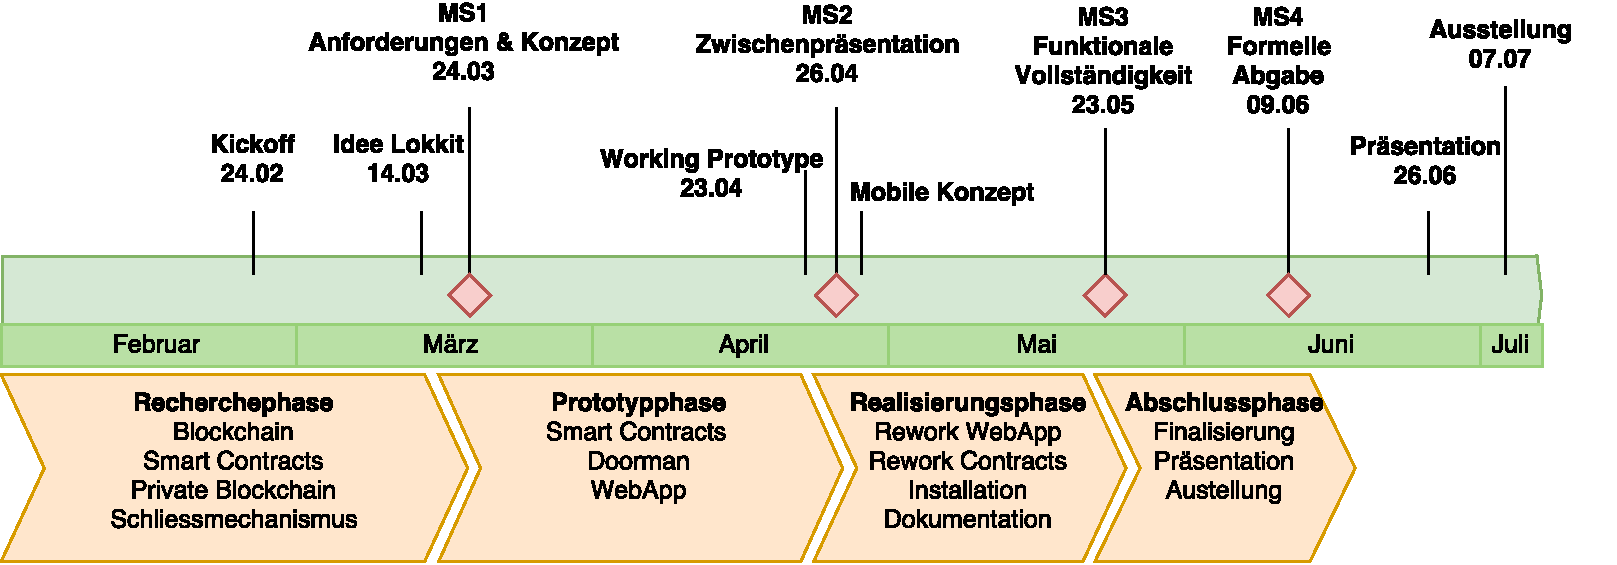
\includegraphics[width=.95\textwidth]{Zeitachse}
\caption{Zeitachse mit Projektphasen und Meilensteine}
\label{fig:Zeitachse mit Projektphasen und Meilensteine}
\end{figure}


\#todo: plan inkl. meilensteine einfügen (aus mid term präsi, evtl updaten)

\paragraph{Initialisierung 24. März}
\label{pm_para:Initialisierung}
Bis am 24. März war die Recherche und Ausarbeitung einer konkreten Aufgabenstellung geplant, die anschliessend implementiert wird. Ein Grobkonzept inklusive Anforderungen für einen Prototyp sollten vorliegen.

Diese Aufgabenstellung wurde am 13. März dem Auftraggeber mitgeteilt und am 14. März besprochen und angenommen (\#todo: siehe email vom 14.3)

\#todo: kommentare des Auftraggebers: siehe Notizen

\#todo: verweis auf requirements für prototyp

\paragraph{Zwischenpräsentation 26. April}
(Prototyp lauffähig) Während er Prototypphase sollte ein definierter Prototyp implementiert werden, der an der Zwischenpräsentation am 26. April vorgeführt werden kann. Dies diente zum einen der raschen Entwicklung einer demonstrierbaren Funktionalität an den Auftraggeber und zum anderen dem Sammeln von konkreten Erfahrungen für das Projektteam im Bereich der Blockchain Technologien. Diese Erfahrungen konnten in der darauf folgenden Phase gewinnbringend eingesetzt und zur Verbesserung der bestehenden Funktionalität verwendet werden.

Der Prototyp mit komplettem Systemdurchstich konnte demonstriert werden. Durch eine Webapp und lokal laufender Ethereum Node wurde demonstriert, dass die Smart Contracts sowie die Anbindung an die private Blockchain funktioniert und auch die Echtzeitkommunikation lauffähig ist.

\paragraph{Formelle Abgabe 9. Juni}
(Dokumentation abgabefertig \& Demonstrator lauffähig) Das Ende des Projektes war der 9. Juni 2017. An diesem Datum sollte der Demonstrator lauffähig, alle Funktionalität dokumentiert und die formellen Testfälle ausgeführt und entsprechend festgehalten sein. 

\#todo: Was hat alles funktioniert, was nicht?

\paragraph{Abschlusspräsentation 26. Juni}
Demonstrator ''gehärtet'' für Abschlusspräsentation und Demonstration (Verbesserungen bei Benutzerfreundlichkeit, Stabilität o.Ä.)
Funktional ist der Demonstrator und jegliche Dokumentation dessen abgeschlossen. Arbeiten, die am Demonstrator nach der Abgabe der Dokumentation gemacht wurden, beschränken sich nur auf den vorführbaren Wert für die Abschlusspräsentation und die Demonstration am 7. Juli.

\#todo: Hier werden wir allfällige weitere Änderungen referenzieren und als v1.1 an der Abschlusspräsi abgeben. Auch Geänderte Dokumente werden als v1.1 abgegeben.

\subsubsection{Recherchephase \emph{Initialisierungsphase}}
\label{pm_subsubsec:Recherchephase}
Im Rahmen des Kick-Off Meetings am 24. Februar übergab der Auftraggeber dem Projektteam den Projektauftrag für einen Demonstrator. Daraufhin wurde ein Rahmenplan erstellt und Meilensteine definiert. In der Recherchephase sollten bestehende Blockchain und IoT Technologien analysiert werden und darauf basierend ein Konzept für einen Demonstrator mit dem Auftraggeber besprochen und definiert werden.

\subsubsection{Prototypphase \emph{Konzeptionsphase}}
\label{pm_subsubsec:Prototypphase}
Das Ziel dieser Phase war es, einen Prototyp zu erstellen, der aufzeigt, dass die Aufgabenstellung so umgesetzt werden kann, wie sie im Konzept definiert wurde. Dabei ist zu beachten, dass das Blockchain Thema im Vordergrund stand. Bei der Umsetzung des Prototyps wurde nach dem explorativen Prinzip gearbeitet, wobei in Intervallen von einer Woche im Projektteam die momentane Situation analysiert und weitere Schritte festgelegt wurden. Hierbei griff das Projektteam sich verändernde Abhängigkeiten (siehe geth 1.6.1\^, status-im, web3 (whisper 5)) auf und versuchte ein limitiertes Set an Anforderungen für den Prototypen zu implementieren, um für die Realisierungsphase eine adäquate zusätzliche Menge Anforderungen definieren zu können.

Am Ende dieser Phase fand die Midterm Präsentation statt, bei der dem Auftraggeber die bisherigen Erfolge, namentlich der Prototyp, vorgeführt wurde. Diese Präsentation diente auch der Besprechung weiterer Anforderungen für die Realisierungsphase, in der der Demonstrator, inklusive der IoT Aspekte, vollumfänglich implementiert werden soll.

\subsubsection{Realisierungsphase}
\label{pm_subsubsec:Realisierungsphase}
Durch die Vorarbeit in den Recherche- und Prototyp- Phasen konnte für die Realisierungsphase eine Menge von Anforderungen definiert werden, die es zu implementieren gilt. Die Vorgehensweise in dieser Phase lehnt sich an das iterativ-inkrementelle Modell von SoDa an, verzichtet jedoch auf explizite Sprints und pflegt keine unterschiedlichen Product- und Sprintbacklogs. Wie auch in der Prototypphase wurden wöchentlich die Arbeiten besprochen und ad-hoc neue Prioritäten für die nächste Woche, basierend auf den noch offenen Anforderungen, definiert. Dies war möglich, da alle Anforderungen bereits in der Recherchephase definiert wurden. Technisch detaillierte User Stories zu definieren war nicht angebracht, da das know-how zur genügenden Fomrulierung solcher grösstenteils während der Realisierung erarbeitet werden musste. Auch die Grösse des Teams und die limitierte Zeitspanne rechtfertigt diese abgespeckte Interpretation von SoDa.

\subsubsection{Projektabschlussphase}
\label{pm_subsubsec:Projektabschlussphase}
In der Projektabschlussphase wurden letzte Integrationstests ausgeführt, um die volle Funktionsfähigkeit des Demonstrators sicherzustellen und allfällige Abweichungen von der Konzeption zu dokumentieren. Weiter wurden die formalen Dokumente vervollständigt und abgeschlossen.

\subsection{Meilensteine}
Am Ende jeder Phase wurde ein Meilenstein mit erwarteten Resultaten definiert.

\subsection{Projektkontrolle}
Der Fortschritt wurde per eMail und in der Midterm Präsentation vom Projektteam an den Auftraggeber kommuniziert.

IST vs SOLL zustand und Massnahmen. (fakultativ)
bspw. bei Rückstand im Projektplan o.Ä.


\subsection{Verantwortlichkeiten}
Dominik Hirzel
\begin{itemize}
    \item Smart Contracts
    \item Android App
    \item Dokumentation
\end{itemize}

\noindent 
Andreas Schmid
\begin{itemize}
    \item Blockchain
    \item IoT
    \item Webapp
    \item Doorman
\end{itemize}


\section{Risikomanagement}
Das Risikomanagement wurde basierend auf der gängigen, und auch in SoDa definierten, Matrixmethode. Die horizontale Achse der Matrix entspricht der Auftretenswahrscheinlichkeit des Risikos, die vertikale Achse spiegelt die Schwere der Auswirkung wieder. Eine höhere Zahl bedeutet hierbei häufiger und schlimmer. Befindet sich die Wahrscheinlichkeit oder die Auswirkung eines Risikos im roten Bereich (vgl. \ref{tbl:Risikomatrix_Leer}), muss mindestens eine Mitigationsmassnahe getroffen werden, um die entsprechende Eigenschaft in den gelben Bereich zu verschieben. Bestenfalls würden Risiken durch besagte Massnahmen eliminiert werden.

\begin{table}[]
\centering
\caption{Risikomatrix Leer}
\label{tbl:Risikomatrix_Leer}
\begin{tabular}{@{}ccccccc@{}}
 & 5 & \cellcolor[HTML]{DF8181} & \cellcolor[HTML]{DF8181} & \cellcolor[HTML]{DF8181} & \cellcolor[HTML]{DF8181} & \cellcolor[HTML]{DF8181} \\
 & 4 & \cellcolor[HTML]{FFFA8F} & \cellcolor[HTML]{FFFA8F} & \cellcolor[HTML]{FFFA8F} & \cellcolor[HTML]{DF8181} & \cellcolor[HTML]{DF8181} \\
 & 3 & \cellcolor[HTML]{92D050} & \cellcolor[HTML]{FFFA8F} & \cellcolor[HTML]{FFFA8F} & \cellcolor[HTML]{FFFA8F} & \cellcolor[HTML]{DF8181} \\
 & 2 & \cellcolor[HTML]{92D050} & \cellcolor[HTML]{92D050} & \cellcolor[HTML]{FFFA8F} & \cellcolor[HTML]{FFFA8F} & \cellcolor[HTML]{DF8181} \\
\multirow{-5}{*}{\rotatebox[origin=c]{90}{Auswirkung}} & 1 & \cellcolor[HTML]{92D050} & \cellcolor[HTML]{92D050} & \cellcolor[HTML]{92D050} & \cellcolor[HTML]{FFFA8F} & \cellcolor[HTML]{DF8181} \\
                             &   & 1                        & 2                        & 3                        & 4                        & 5                        \\
                             &   & \multicolumn{5}{c}{Wahrscheinlichkeit}                                                                                              
\end{tabular}
\end{table}

\subsection{Übersicht}
Risiken werden für jede Phase als Übersicht vollumfänglich tabellarisch festgehalten. D.h., dass nicht nur neue Risiken erfasst sondern auch bestehende Risiken neu evaluiert (oder gestrichen) werden. Hierbei wird bewusst gewisse Redundanz zu Gunsten der Vollständigkeit auf einen Blick in Kauf genommen. Die Risiken werden mit einer Nummer und einem Namen zur einfacheren Identifikation versehen. Eine ausführliche Beschreibung der Risiken, eine Begründung für die Kategorisierung, allfällige Mitigationsmassnahmen und Massnahmen bei Eintreffen des Risikos werden anschliessend gelistet, sollte dies benötigt werden. Die Risiken werden in der Matrix vor und nach der Mitigationsmassnhamen dargestellt. Dabei ist die betonte Zahl (bspw. \emph{1}) die Kategorisierung des Risikos vor und die voll schwarze Zahl (bspw. 1) dieselbe nach den Mitigationsmassnahmen. Sollte keine Massnahmen getroffen worden sein, wird die kursive Zahl ausgelassen. 

\subsection{Risiken Recherchephase}
Während der Recherchephase waren die hauptsächlichen Risiken, dass der frühe Entwicklungsstand aller Blockchain Implementationen nicht die volle Funktionalität bietet, die für einen adäquaten Demonstrator benötigt wird.

\begin{table}[H]
\centering
\caption{Risiken Recherchephase}
\label{tbl:Risiken_Recherche}
\begin{tabular}{lL{8cm}lll}
\toprule
Nr. & Risiko & A & W & Status \\ \midrule
1  & Keine Blockchain Implementation unterstützt Funktionalität für den Demonstrator & 5 & 3 & Neu \\\midrule
2  & Höhere Belastung des Projektteams durch Berufstätigkeit & 2 & 2 & Neu    \\\midrule
\end{tabular}
\end{table}

\begin{table}[H]
\centering
\caption{Risikomatrix Recherche}
\label{tbl:Risikomatrix_Recherche}
\begin{tabular}{@{}ccccccc@{}}
 & 5 & \cellcolor[HTML]{DF8181} & \cellcolor[HTML]{DF8181} & \cellcolor[HTML]{DF8181}1 & \cellcolor[HTML]{DF8181} & \cellcolor[HTML]{DF8181} \\
 & 4 & \cellcolor[HTML]{FFFA8F} & \cellcolor[HTML]{FFFA8F} & \cellcolor[HTML]{FFFA8F} & \cellcolor[HTML]{DF8181} & \cellcolor[HTML]{DF8181} \\
 & 3 & \cellcolor[HTML]{92D050} & \cellcolor[HTML]{FFFA8F} & \cellcolor[HTML]{FFFA8F} & \cellcolor[HTML]{FFFA8F} & \cellcolor[HTML]{DF8181} \\
 & 2 & \cellcolor[HTML]{92D050} & \cellcolor[HTML]{92D050}2 & \cellcolor[HTML]{FFFA8F} & \cellcolor[HTML]{FFFA8F} & \cellcolor[HTML]{DF8181} \\
\multirow{-5}{*}{\rotatebox[origin=c]{90}{Auswirkung}} & 1 & \cellcolor[HTML]{92D050} & \cellcolor[HTML]{92D050} & \cellcolor[HTML]{92D050} & \cellcolor[HTML]{FFFA8F} & \cellcolor[HTML]{DF8181} \\
                             &   & 1                        & 2                        & 3                        & 4                        & 5                        \\
                             &   & \multicolumn{5}{c}{Wahrscheinlichkeit}                                                                                              
\end{tabular}
\end{table}

\paragraph{Risiko 1}
Sollte eine angedachte Funktionalität von keiner Blockchain Implementation unterstützt werden, kann der Demonstrator nicht wie geplant implementiert werden.
\subparagraph{Mitigation}
Präventierende Massnahmen können hier nicht getroffen werden, da die Anforderungen während der Recherchephase basierend auf zur Verfügung stehender Technologie gemacht werden.
\subparagraph{Sofortmassnahmen}
Sollte aufgrund mangelnder Funktionalität der Blockchain Implementationen ein Demonstrator nicht mit angebrachter Funktionalität spezifizierbar sein, werden die Anforderungen an den Demonstrator vereinfacht. Ebenfalls wird mit dem Auftraggeber und Betreuer Kontakt aufgenommen, um die Limitationen in der selbst definierten Aufgabenstellung zu kommunizieren und Alternativen dazu zu suchen.

\subsection{Risiken Prototypphase}
Während der Prototypphase waren die hauptsächlichen Risiken, dass die laufende Entwicklung an \emph{geth} die zu implementierende Funktionalität für den Demonstrator einschränken kann.

\begin{table}[H]
\centering
\caption{Risiken Prototypphase}
\label{tbl:Risiken_Prototyp}
\begin{tabular}{lL{8cm}lll}
\toprule
Nr. & Risiko & A & W & Status \\ \midrule
1  & \sout{Keine Blockchain Implementation unterstützt Funktionalität für den Demonstrator} & 0 & 0 & eliminiert \\\midrule
2  & Höhere Belastung des Projektteams durch Berufstätigkeit & 2 & 2 & erkannt    \\\midrule
3  & Stabilität von geth & 5 & 4 & Neu    \\\midrule
4  & Mangelnde Dokumentation und Hilfestellung zu geth & 4 & 4 & Neu    \\\midrule
\end{tabular}
\end{table}

\begin{table}[H]
\centering
\caption{Risikomatrix Prototypphase}
\label{tbl:Risikomatrix_Prototyp}
\begin{tabular}{@{}ccccccc@{}}
 & 5 & \cellcolor[HTML]{DF8181} & \cellcolor[HTML]{DF8181} & \cellcolor[HTML]{DF8181}\emph{3} & \cellcolor[HTML]{DF8181} & \cellcolor[HTML]{DF8181} \\
 & 4 & \cellcolor[HTML]{FFFA8F} & \cellcolor[HTML]{FFFA8F} & \cellcolor[HTML]{FFFA8F} & \cellcolor[HTML]{DF8181}\emph{4} & \cellcolor[HTML]{DF8181} \\
 & 3 & \cellcolor[HTML]{92D050} & \cellcolor[HTML]{FFFA8F} & \cellcolor[HTML]{FFFA8F}3 & \cellcolor[HTML]{FFFA8F} & \cellcolor[HTML]{DF8181} \\
 & 2 & \cellcolor[HTML]{92D050} & \cellcolor[HTML]{92D050}2 & \cellcolor[HTML]{FFFA8F} & \cellcolor[HTML]{FFFA8F}4 & \cellcolor[HTML]{DF8181} \\
\multirow{-5}{*}{\rotatebox[origin=c]{90}{Auswirkung}} & 1 & \cellcolor[HTML]{92D050} & \cellcolor[HTML]{92D050} & \cellcolor[HTML]{92D050} & \cellcolor[HTML]{FFFA8F} & \cellcolor[HTML]{DF8181} \\
                             &   & 1                        & 2                        & 3                        & 4                        & 5                        \\
                             &   & \multicolumn{5}{c}{Wahrscheinlichkeit}                                                                                              
\end{tabular}
\end{table}

\paragraph{Risiko 1}
Die Implementation geth unterstützt das Ethereum Protokoll, private Netzwerke, Light Nodes (vgl. \ref{para:Light_Node}) (experimentell) und Smart Contracts und kann somit für einen Demonstrator verwendet werden.

\paragraph{Risiko 3}
Da an geth stark entwickelt wird und auch das Ethereum Protokoll Änderungen unterzogen wird, muss damit gerechnet werden, dass die Implementation und auch die Spezifikation geändert werden können. Auch sind kritische Fehler, die die Verwendung von geth oder einzelnen Funktionalitäten verhindern, zu beachten.\cite[EIPs]{github.com/ethereum}
\subparagraph{Mitigation}
Durch ständiges Updaten der Abhängigkeiten kann sichergestellt werden, dass stets eine unterstützte Version des Ethereum Protokolls benutzen wird.
\subparagraph{Sofortmassnahmen}
Das Projektteam integriert sich aktiv in der ethereum Entwicklercommunity durch Teilnahme am gitter chat und Rückmeldung von Fehlern in \emph{geth}.

\paragraph{Risiko 4}
Während der Recherchephase wurde festgestellt, dass die Dokumentation von geth und Teilfunktionen davon nicht immer dem aktuellsten Entwicklungsstand entsprachen. Da an geth stark entwickelt wird und auch das Ethereum Protokoll Änderungen unterzogen wird, muss damit gerechnet werden, dass die Implementation und auch die Spezifikation geändert werden können.
\subparagraph{Mitigation}
Durch ständiges Updaten der Abhängigkeiten kann sichergestellt werden, dass stets eine unterstützte Version des Ethereum Protokolls benutzen wird. Das Projektteam integriert sich auch aktiv in der ethereum Entwicklercommunity durch Teilnahme am gitter chat und Rückmeldung von Fehlern in geht.
\subparagraph{Sofortmassnahmen}
Das Projektteam integriert sich aktiv in der Ethereum Entwicklercommunity durch Teilnahme am gitter chat und Rückmeldung von Fehlern in geth.


\subsection{Risiken Realisierungsphase}
Während der Realisierungsphase waren die hauptsächlichen Risiken, dass die laufende Entwicklung an geth die zu implementierende Funktionalität für den Demonstrator einschränken kann.

\begin{table}[H]
\centering
\caption{Risiken Realisierung}
\label{tbl:Risiken_Realisierung}
\begin{tabular}{lL{8cm}lll}
\toprule
Nr. & Risiko & A & W & Status \\ \midrule
1  & \sout{Keine Blockchain Implementation unterstützt Funktionalität für den Demonstrator} & 0 & 0 & eliminiert \\\midrule
2  & Höhere Belastung des Projektteams durch Berufstätigkeit & 4 & 3 & erkannt    \\\midrule
3  & Stabilität von geth & 5 & 4 & erkannt    \\\midrule
4  & Mangelnde Dokumentation und Hilfestellung zu geth & 4 & 4 & erkannt    \\\midrule
5  & Mangelndes Wissen im Bereich Hardware \& Elektronik & 3 & 3 & neu    \\\midrule
6  & Schliessmechanismen können nicht reverse engineered werden & 5 & 2 & neu    \\\midrule
7  & Einzelteile für den Demonstrator können nicht rechtzeitig geliefert werden & 3 & 4 & neu    \\\midrule
\end{tabular}
\end{table}

\begin{table}[H]
\centering
\caption{Risikomatrix Realisierungphase}
\label{tbl:Risikomatrix_Realisierung}
\begin{tabular}{@{}ccccccc@{}}
 & 5 & \cellcolor[HTML]{DF8181} & \cellcolor[HTML]{DF8181}\emph{6} & \cellcolor[HTML]{DF8181}\emph{3} & \cellcolor[HTML]{DF8181} & \cellcolor[HTML]{DF8181} \\
 & 4 & \cellcolor[HTML]{FFFA8F} & \cellcolor[HTML]{FFFA8F} & \cellcolor[HTML]{FFFA8F}\emph{2},\emph{7} & \cellcolor[HTML]{DF8181}\emph{4} & \cellcolor[HTML]{DF8181} \\
 & 3 & \cellcolor[HTML]{92D050} & \cellcolor[HTML]{FFFA8F} & \cellcolor[HTML]{FFFA8F}3,\emph{5} & \cellcolor[HTML]{FFFA8F} & \cellcolor[HTML]{DF8181} \\
 & 2 & \cellcolor[HTML]{92D050} & \cellcolor[HTML]{92D050}2,5 & \cellcolor[HTML]{FFFA8F} & \cellcolor[HTML]{FFFA8F}4 & \cellcolor[HTML]{DF8181} \\
\multirow{-5}{*}{\rotatebox[origin=c]{90}{Auswirkung}} & 1 & \cellcolor[HTML]{92D050}6 & \cellcolor[HTML]{92D050} & \cellcolor[HTML]{92D050} & \cellcolor[HTML]{FFFA8F} & \cellcolor[HTML]{DF8181} \\
                             &   & 1                        & 2                        & 3                        & 4                        & 5                        \\
                             &   & \multicolumn{5}{c}{Wahrscheinlichkeit}
\end{tabular}
\end{table}

\paragraph{Risiko 2}
Da die Realisierungsphase sehr viel Zeit beansprucht wird dieses Risiko höher bewertet.
\subparagraph{Mitigation}
Alle Beteiligten des Projektteams führen eine transparente Beziehung zu ihrem Arbeitgeber bezüglich ihrem Studium. Die Arbeitgeber unterstützen die Beteiligten des Projektteams in ihrem Studium. Durch frühzeitige Kommunikation mit dem Arbeitgeber bezüglich fixen Terminen oder Projektabschlussphase\footnote{Namentlich der Präsentationterminen, sowie der Intensivwoche anfangs Juni.} wird diesem Risiko entgegengewirkt.
\subparagraph{Sofortmassnahmen}
Rasche Kommunikation mit dem Projektteam und Kompensation der verlorenen Zeit zu einem späteren Zeitpunkt.

\paragraph{Risiko 3}
Auch in der Realisierungsphase wurde weiter stark an geth und dem Ethereum Protokoll entwickelt. Somit muss damit gerechnet werden, dass die Implementation und auch die Spezifikation geändert werden können. Auch sind kritische Fehler, die die Verwendung von geth oder einzelnen Funktionalitäten verhindern, zu beachten.\cite[EIPs]{github.com/ethereum}
\subparagraph{Mitigation}
Durch ständiges Updaten der Abhängigkeiten kann sichergestellt werden, dass stets eine unterstützte Version des Ethereum Protokolls benutzen wird.
\subparagraph{Sofortmassnahmen}
Das Projektteam integriert sich aktiv in der Ethereum Entwicklercommunity durch Teilnahme am gitter chat und Rückmeldung von Fehlern in geht.

\paragraph{Risiko 4}
Während der Recherchephase wurde festgestellt, dass die Dokumentation von geth und Teilfunktionen davon nicht immer dem aktuellsten Entwicklungsstand entsprachen. Da an geth stark entwickelt wird und auch das Ethereum Protokoll Änderungen unterzogen wird, muss damit gerechnet werden, dass die Implementation und auch die Spezifikation geändert werden können.
\subparagraph{Mitigation}
Durch ständiges Updaten der Abhängigkeiten kann sichergestellt werden, dass stets eine unterstützte Version des Ethereum Protokolls benutzen wird. Das Projektteam integriert sich auch aktiv in der ethereum Entwicklercommunity durch Teilnahme am gitter chat und Rückmeldung von Fehlern in geht.
\subparagraph{Sofortmassnahmen}
Das Projektteam integriert sich aktiv in der Ethereum Entwicklercommunity durch Teilnahme am gitter chat und Rückmeldung von Fehlern in geth.

\paragraph{Risiko 5}
Das Projektteam besteht aus Studierenden im Bereich Informatik. Daher kann nicht ausgeschlossen werden, dass für die Implementation des IoT Demonstrators Fachwissen im Bereich Elektronik und Maschinenbau fehlt.
\subparagraph{Mitigation}
Durch vergangene Arbeit in privaten Projekten mit elektronischen Elementen hat das Projektteam begrenzte Erfahrung. Basierend auf diesen bestehenden Kenntnissen kann weiteres Wissen erworben werden. 
\subparagraph{Sofortmassnahmen}
Sollte das benötigte Fachwissen nicht vorhanden sein und nicht in akzeptablem Rahmen aufgebaut werden können, werden Kommilitonen aus den Studienbereich Elektronik und/oder Maschinenbau um Hilfe gebeten, die aus den Fächern PREN1 und PREN2 bekannt sind.

\paragraph{Risiko 6}
Die zur Verfügung gestellten Schliessmechanismen\footnote{Namentlich: Noke und eqiva(vgl. http://www.pearl.de/a-ZX2430-3112.shtml;jsessionid=kCB676D6AFB1D502B2E4B74AA6E98113E)} benutzen teils proprietäre Kommunikationsprotokolle oder sind offiziell nur über ein App ansprechbar.
\subparagraph{Mitigation}
Mit den Herstellern der Schliessmechanismen soll Kontakt aufgenommen werden, um die Wahrscheinlichkeit zu erhöhen, dass diese von lokkit angesprochen werden können. Sollte die Möglichkeit zur Ansprechung der Mechanismen durch Massnahmen des Herstellers erschwert oder verhindert werden, würde der jeweilige Mechanismus zugunsten eines selbst entworfenen Schliessmechanismus nicht weiter verfolgt.
\subparagraph{Sofortmassnahmen}
Da ohnehin ein selbst entworfener Schliessmechanismus eingebaut wird, kann dieser in mehrfacher Ausführung eingebaut werden.

\paragraph{Risiko 7}
Der Demonstrator wird ebenfalls vom Projektteam implementiert. Schliessmechanismen sind unterschiedliche erhältlich, jedoch müssen diese auch mit dem Schliessfachschrank kompatibel sein.
\subparagraph{Mitigation}
Für Teile, deren Lieferfrist einen akzeptable Termin überdauert, sollen Alternativen gesucht werden.
\subparagraph{Sofortmassnahmen}
Da ohnehin ein selbst entworfener Schliessmechanismus eingebaut wird, kann dieser in mehrfacher Ausführung eingebaut werden.


\subsection{Risiken Projektabschlussphase}
In der Projektabschlussphase wird vermehrt ein Augenmerk auf die formellen Dokumente gelegt und somit treffen die meisten technischen Risiken nicht mehr zu.

\begin{table}[H]
\centering
\caption{Risiken Realisierung}
\label{tbl:Risiken_Realisierung}
\begin{tabular}{lL{8cm}lll}
\toprule
Nr. & Risiko & A & W & Status \\ \midrule
1  & \sout{Keine Blockchain Implementation unterstützt Funktionalität für den Demonstrator} & 0 & 0 & eliminiert \\\midrule
2  & Höhere Belastung des Projektteams durch Berufstätigkeit & 4 & 3 & erkannt    \\\midrule
3  & \sout{Stabilität von geth} & 0 & 0 & eliminiert    \\\midrule
4  & \sout{Mangelnde Dokumentation und Hilfestellung zu geth} & 0 & 0 & eliminiert    \\\midrule
5  & \sout{Mangelndes Wissen im Bereich Hardware \& Elektronik} & 0 & 0 & eliminiert    \\\midrule
6  & \sout{Schliessmechanismen können nicht reverse engineered werden} & 0 & 0 & eliminiert    \\\midrule
7  & \sout{Einzelteile für den Demonstrator können nicht rechtzeitig geliefert werden} & 0 & 0 & eliminiert    \\\midrule
\end{tabular}
\end{table}

\begin{table}[H]
\centering
\caption{Risikomatrix Realisierungphase}
\label{tbl:Risikomatrix_Realisierung}
\begin{tabular}{@{}ccccccc@{}}
 & 5 & \cellcolor[HTML]{DF8181} & \cellcolor[HTML]{DF8181} & \cellcolor[HTML]{DF8181} & \cellcolor[HTML]{DF8181} & \cellcolor[HTML]{DF8181} \\
 & 4 & \cellcolor[HTML]{FFFA8F} & \cellcolor[HTML]{FFFA8F} & \cellcolor[HTML]{FFFA8F}\emph{2} & \cellcolor[HTML]{DF8181} & \cellcolor[HTML]{DF8181} \\
 & 3 & \cellcolor[HTML]{92D050} & \cellcolor[HTML]{FFFA8F} & \cellcolor[HTML]{FFFA8F} & \cellcolor[HTML]{FFFA8F} & \cellcolor[HTML]{DF8181} \\
 & 2 & \cellcolor[HTML]{92D050} & \cellcolor[HTML]{92D050}2 & \cellcolor[HTML]{FFFA8F} & \cellcolor[HTML]{FFFA8F} & \cellcolor[HTML]{DF8181} \\
\multirow{-5}{*}{\rotatebox[origin=c]{90}{Auswirkung}} & 1 & \cellcolor[HTML]{92D050} & \cellcolor[HTML]{92D050} & \cellcolor[HTML]{92D050} & \cellcolor[HTML]{FFFA8F} & \cellcolor[HTML]{DF8181} \\
                             &   & 1                        & 2                        & 3                        & 4                        & 5                        \\
                             &   & \multicolumn{5}{c}{Wahrscheinlichkeit}
\end{tabular}
\end{table}

\paragraph{Risiko 3}
Durch Abschluss der Realisierungsphase trifft dies nicht mehr zu.
\paragraph{Risiko 4}
Durch Abschluss der Realisierungsphase trifft dies nicht mehr zu.
\paragraph{Risiko 5}
Durch Abschluss der Realisierungsphase trifft dies nicht mehr zu.
\paragraph{Risiko 6}
Durch Abschluss der Realisierungsphase trifft dies nicht mehr zu.
\paragraph{Risiko 7}
Durch Abschluss der Realisierungsphase trifft dies nicht mehr zu.

\section{Projektunterstützung}
\subsection{Tools}
github, sharelatex, draw.io, inkscape, vim, visual studio code, android studio (full suite), 

\subsection{Konfigurationsmanagement}
\#TODO:Zusammenspiel der Versionen der Komponenten. --> Da nur eine Version veröffentlich wird, ist dies warscheinlich alles V1.0.0.
\chapter{Testing}

Dieses Dokument beschreibt das Testkonzept, das verfolgt wurde, um sicher zu stellen, dass das System wie angedacht funktioniert.

\subsection{Teststrategie}
Das System hat einen hoch komplexen Aufgbau und viele einzelne Komponenten. Umso wichtiger und komplizierter ist auch das Testing. Das Projekt wird auf drei Ebenen getestet. 

\vspace{.3cm}
\begin{description}
    \item[Unittests] Diese Tests sind vorallem während der Entwicklung einer Komponente wichtig.
    \item[Integrationstests] Einige Komponenten sind stark von der Blockchain abhängig und müssen daher mit einer laufenden Blockchain Node getestet werden. Um dies zu vereinfachen wurde ein Dockerimage für eine lokale Blockchain erstellt.
    \item [Systemtests] Diese Tests testen das ganze System, inklusive aller Komponenten und der Blockchain. Mittels diesen Tests werden alle Use Cases validiert. Diese Tests gelten auch als Abnahmetests, um die Gesamtfunktionalität zu garantieren.
\end{description}
\noindent
In den nachfolgenden Kapiteln werden die einzlnen Unittests, Integrationstests und Systemtests aufgelistet.

\subsection{Unittest}

\subsubsection{Smart Contract}
Die Tests können mit dem Befehl \emph{truffle test} auseführt werden.

\begin{table}[H]
\centering
\caption{Unittests des Smart Contracts Rentable}
\label{my-label}
\begin{tabular}{@{}L{.5cm}L{6cm}L{6cm}@{}}
\toprule
Nr. & 
Testname & 
Beschreibung 
\\ \midrule
1
& costPerSecond contract should be 7 
& Testet das Setzen von costPerSecond und dessen Berechnung 
\\ \midrule
2   
& descritption of contract should be 'leDescription'         
& Testet das \emph{Description}-Feld
\\ \midrule
3   
& location of contract should be 'leLocation'         
& Testet das \emph{Location}-Feld 
\\ \midrule
4   
& deposit of contract should be 500"         
& Testet das \emph{deposit}-Feld 
\\ \midrule
5   
& reserve (rent) the rentable         
& Testet die die \emph{reservedBetween} Funktion 
\\ \midrule
6   
& rent and check if reserved between         
& Testet die die \emph{rent} Funktion 
\\ \bottomrule
\end{tabular}
\end{table}

\begin{table}[H]
\centering
\caption{Unittests des Smart Contracts RentableDiscovery}
\label{my-label}
\begin{tabular}{@{}L{.5cm}L{6cm}L{6cm}@{}}
\toprule
Nr. & 
Testname & 
Beschreibung 
\\ \midrule
1
& can create contract using factory method
& Testet das Erzeugen von neuen \emph{Rentables} mittels Discovery Contract
\\ \bottomrule
\end{tabular}
\end{table}
\subsection{Integrationstests}
Die Integrationstests testen die einzelnen Komponenten gegen die Blockchain. 

\subsubsection{Doorman}

\paragraph{Voraussetzungen}

Um die Integrationstests von Doorman auszuführen muss folgendes Setup durchgeführt werden:

\begin{itemize}
    \item Auschecken der Doorman Resourcen
    \item Installieren der Abhängigkeiten
    \item Starten des Ethereum Nodes mittels Docker
    \item Veröffentlichen des Smart Contracts via truffle 
\end{itemize}

Danach können die Testfälle durchgespielt werden.
    
\begin{table}[H]
\centering
\caption{Test \#1: Starten von Doorman}
\label{my-label}
\begin{tabular}{@{}L{1.6cm}L{11cm}@{}}
\toprule
\textbf{Test \#1}
& Starten von Doorman mit Referenz zum veröffentlichten Contract
\\ \midrule
\textbf{Ablauf}
& 
\begin{enumerate}
    \item Eintragen der Addresse des veröffentlichten Contracts im Config file von Doorman
    \item Starten des Doormans
\end{enumerate}
\\ \midrule
\textbf{Ergebnis}
& Doorman startet und gibt Details zu allen Rentables aus, auf deren Whispers gehört werden soll.

\\ \bottomrule
\end{tabular}
\end{table}

\begin{table}[H]
\centering
\caption{Test \#2: Doorman emfpängt Lock/Unlock-Befehl vom aktuellen Mieter}
\label{my-label}
\begin{tabular}{@{}L{1.6cm}L{11cm}@{}}
\toprule
\textbf{Test \#2}
& Doorman emfpängt Lock/Unlock-Befehl vom aktuellen Mieter
\\ \midrule
\textbf{Ablauf}
& 
\begin{enumerate}
    \item Mittels Truffle das Rentable für 5 min mieten
    \item Danach den Lock-Befehl ausführen
    \item Danach den Unlock-Befehl ausführen
\end{enumerate}
\\ \midrule
\textbf{Ergebnis}
& Doorman startet und gibt eine Erfolgsmeldung für das jeweilige Rentable aus.

\\ \bottomrule
\end{tabular}
\end{table}

\begin{table}[H]
\centering
\caption{Test \#3: Doorman emfpängt Lock/Unlock-Befehl von unbekanntem Account}
\label{my-label}
\begin{tabular}{@{}L{1.6cm}L{11cm}@{}}
\toprule
\textbf{Test \#3}
& Doorman emfpängt Lock/Unlock-Befehl von unbekanntem Account
\\ \midrule
\textbf{Ablauf}
& 
\begin{enumerate}
    \item Neuen Account auf der Node erstellen
    \item Lock Befehl signiert mit dem neuen Account absenden
    \item Unlock Befehl signiert mit dem neuen Account absenden
\end{enumerate}
\\ \midrule
\textbf{Ergebnis}
& Doorman startet und gibt eine Fehlermeldung für den unbekannten account aus.

\\ \bottomrule
\end{tabular}
\end{table}

\subsubsection{Webapp}

\paragraph{Voraussetzungen}

Um die Integrationstests von der Webapp auszuführen muss folgendes Setup durchgeführt werden:

\begin{itemize}
    \item Auschecken der Webapp Resourcen
    \item Installieren der Abhängigkeiten
    \item Starten des Ethereum Nodes mittels Docker
    \item Starten der Webapp
    \item Veröffentlichen des Smart Contracts via truffle 
\end{itemize}

Danach können die Testfälle durchgespielt werden.


\begin{table}[H]
\centering
\caption{Test \#1: Hinzufügen eines Rentables }
\label{my-label}
\begin{tabular}{@{}L{1.6cm}L{11cm}@{}}
\toprule
\textbf{Test \#1}
& Hinzufügen eines Rentables
\\ \midrule
\textbf{Ablauf}
& 
\begin{enumerate}
    \item Füge das Rentable hinzu
    \item Schliesse den Browser und starte erneut
    \item Überprüfe, ob das Rentable noch hinzugefügt ist
\end{enumerate}
\\ \midrule
\textbf{Ergebnis}
& Das Rentable ist immer noch hinzugefügt.
\\ \bottomrule
\end{tabular}
\end{table}


\begin{table}[H]
\centering
\caption{Test \#2: Reservieren eines Rentables }
\label{my-label}
\begin{tabular}{@{}L{1.6cm}L{11cm}@{}}
\toprule
\textbf{Test \#2}
& Reservieren eines Rentables
\\ \midrule
\textbf{Ablauf}
& 
\begin{enumerate}
    \item Reserviere ein Rentable für 2 Minuten
    \item Überprüfe, ob die Reservations erfolgreich erscheint.
    \item Überprüfe, ob nach eintreten der Reservationszeit die Buttons Lock, Unlock erscheinen.
    \item Überprüfe, ob nach Aublauf der Reservation, die Buttons wieder verschwinden
\end{enumerate}
\\ \midrule
\textbf{Ergebnis}
& Die Reservation läuft erfolgreich durch. Beim Anbruch der Reservationsdauer sind Unlock und Lock ersichtlich. Nach Ablauf von ca 2. Minuten verschwinden die Buttons wieder. 
\\ \bottomrule
\end{tabular}
\end{table}


\begin{table}[H]
\centering
\caption{Test \#3: Fehleranzeige bei falscher Reservation}
\label{my-label}
\begin{tabular}{@{}L{1.6cm}L{11cm}@{}}
\toprule
\textbf{Test \#3}
& Fehleranzeige bei falscher Reservation
\\ \midrule
\textbf{Ablauf}
& 
\begin{enumerate}
    \item Reserviere ein Rentable in der Vergangenheit
    \item Überprüfe, ob eine entsprechende Fehlermeldung erscheint
\end{enumerate}
\\ \midrule
\textbf{Ergebnis}
& Das Rentable kann nicht reserviert werden, da eine Reservation in der Vergangenheit nicht möglich ist. 
\\ \bottomrule
\end{tabular}
\end{table}

\begin{table}[H]
\centering
\caption{Test \#4: Fehleranzeige bei Reservation mit Account ohne Ether}
\label{my-label}
\begin{tabular}{@{}L{1.6cm}L{11cm}@{}}
\toprule
\textbf{Test \#4}
& Fehleranzeige bei falscher Reservation
\\ \midrule
\textbf{Ablauf}
& 
\begin{enumerate}
    \item Wechsle den Account zu einem Account der 0 Ether besitzt.
    \item Reserviere ein Rentable in der Zukunft.
    \item Überprüfe, ob eine entsprechende Fehlermeldung erscheint
\end{enumerate}
\\ \midrule
\textbf{Ergebnis}
& Das Rentable kann nicht reserviert werden, da der Account nicht genügend Ether hat.
\\ \bottomrule
\end{tabular}
\end{table}
\subsection{Systemtests}
Die Systemtests testen das Gesamtsystem ausgehend vom Benutzer. Mit diesen Tests ist sichergestellt, dass der Demonstrator funktioniert.

\subsubsection{Voraussetzungen}
Für die folgenden Systemtests wird vorausgesetzt, dass das komplette System installiert und konfiguriert ist. Der Benutzer (Tester) besitzt ein Android Mobile Telefon und kann Applikationen aus dem Internet installieren.

Das Mobile Telefon muss mit dem Demonstrator WLAN verbunden sein.
Für jeden erstellten Account wird Ether vorausgesetzt.


\begin{table}[H]
\centering
\caption{Test \#1: Installieren des Mobile Apps}
\label{my-label}
\begin{tabular}{@{}L{1.6cm}L{11cm}@{}}
\toprule
\textbf{Test \#1}
& Installieren des Mobile Apps
\\ \midrule
\textbf{Ablauf}
& 
\begin{enumerate}
    \item Die Android-App via https://lokkit.io/download installieren
    \item Die Android-App starten (Benutzer muss erstellt werden)
    \item Einloggen des erstellten Benutzers
\end{enumerate}
\\ \midrule
\textbf{Ergebnis}
& Die Android-App ist erfolgreich auf dem Mobile Telefon installiert und kann gestartet werden. Der erstellte Benutzer kann eingeloggt werden.
\\ \bottomrule
\end{tabular}
\end{table}


\begin{table}[H]
\centering
\caption{Test \#2: Reservieren eines Rentables}
\label{my-label}
\begin{tabular}{@{}L{1.6cm}L{11cm}@{}}
\toprule
\textbf{Test \#2}
& Reservieren eines Rentables
\\ \midrule
\textbf{Ablauf}
& 
\begin{enumerate}
    \item Das Rentable über den QR-Code einscannen
    \item Das Rentable reservieren
    \item Ausführen von Lock und Unlock während der Reservationszeit
    \item Rückgabe des Rentables innerhalb der Reservationszeit
\end{enumerate}
\\ \midrule
\textbf{Ergebnis}
& Das Rentable konnte erfolgreich hinzugefügt werden. Die Reservation lief erfolgreich durch. Unlock und Lock haben entsprechend die Türe ge- und entsperrt. Das Rentable konnte erfolgreich zurückgeschoben werden.
\\ \bottomrule
\end{tabular}
\end{table}

\subsection{Testdruchführung am 04.06.2017}

\begin{table}[H]
\centering
\caption{Unittests des Smart Contracts Rentable}
\label{my-label}
\begin{tabular}{@{}L{4.5cm}L{4cm}L{4cm}@{}}
\toprule
Tests &
Tests erfolgreich & 
Tests fehlgeschlagen 
\\ \midrule
7 Unittests 
& 7
& 0
\\ \midrule
3 Integrationstests  
& 3
& 0
\\ \midrule
2 Systemtests
& 2
& 0
\\ \bottomrule
\end{tabular}
\end{table}

\chapter{Installation \& Deployment}
\label{cha:Installation_Deployment}

In den folgenden Abschnitten wird erklärt wie das System aufgesetzt wird. Jede Komponente wird aus den Sourcen gebildet und dann auf den Raspberries installiert. Dazu wird zuerst erklärt wie die Raspberries in Betrieb genommen werden.

\section{Voraussetzungen für das Deployment}
Die nachfolgende Anleitung wurde unter einem aktuellen GNU/Linux System erfolgreich getestet. Grundsätzlich sind andere Systeme wie Windows oder MAC jedoch nicht ausgeschlossen und können für das Deployment ebenfalls verwendet werden. Dies jedoch auf eigene Verantwortung.

Konfigurationsübersicht zu diesem Zeitpunkt

\begin{table}[H]
\centering
\caption{Systemvorausetzungen um das Deployment durchzuführen}
\label{my-label}
\begin{tabular}{@{}lll@{}}
\toprule
Komponente 
& Version               
& Beschreibung                           
\\ \midrule
GNU/Linux  
& Ubuntu 16.04 (Xenial) 
& Basis System für das Deployment        
\\ \midrule
nodejs     
& 7.10.0                
& Voraussetzung für Webapp               
\\ \midrule
npm        
& 4.2.0                 
& Voraussetzung für Webapp               
\\ \midrule
git        
&  2.7.4                
& Zum Auschecken der Sourcen               
\\ \midrule
truffle    
& 3.2.4                 
& Für das Deployment der Smart Contracts 
\\ \midrule
geth       
& 1.6.2                 
& Ethereum Node                          
\\ \midrule
doorman    
&                       
&                           
\\ \midrule
Webapp     
&                       
&                                        
\\ \bottomrule
\end{tabular}
\end{table}

\paragraph{Herunterladen der Resourcen}

Die Lokkit Sourcen können wie folgt heruntergeladen werden:

\begin{lstlisting}[language=bash]
git clone https://github.com/lokkit/lokkit --recursive
\end{lstlisting}

\section{Lokkit Raspberry Pi Image}
Für jedes der drei Raspberry Pi's wurde ein eigenes Image erstellt, welches im Anhang der CD entnommen werden kann. (TODO:) Die Images basiern auf dem offiziellen \emph{Raspbian Jessie Lite} Image \footnote{\url{https://www.raspberrypi.org/downloads/raspbian/}}.

\begin{description}
    \item[Lokkit Image 1] Dieses Image enthält die Konfiguration für den WLAN HotSpot und einen DNS/DHCP Server. Die anderen Raspberries verbinden sich zu diesem.
    \item[Lokkit Image 2] Dieses Image ist so konfiguriert, dass es sich mit dem HotSpot des Master Images verbindet.
    \item[Lokkit Image 3] Dieses Image ist bis auf den Hostnamen identisch mit dem Lokkit Image 2
\end{description}

Alle drei Images können z.B. mit \emph{dd} unter GNU/Linux auf eine MicroSD geflashed werden.

\begin{lstlisting}[language=bash]
dd if=rasp-master.img of=/dev/sdd
dd if=rasp-node1.img of=/dev/sdd
dd if=rasp-node2.img of=/dev/sdd
\end{lstlisting}

Danach können die Raspberries mit dem Image gestartet werden. Nach spätestens 5 Minuten sollte ein HotSpot "lokkit" ersichtlich sein. Das Password lautet "trust-no-one".

Nun kann SSH Verbindung mit z.B. dem Master Rasbperry hergestellt werden.

\begin{lstlisting}[language=bash]
ssh 192.168.0.1 -l pi

\end{lstlisting}

Der User lautet \emph{pi} und das Passwort \emph{TrNoOnJuLo}.

\section{Geth}
\subsection{Installation}
\subsection{Generell}
https://geth.ethereum.org/downloads/

\subsection{Ubuntu}
sudo apt-get install software-properties-common
sudo add-apt-repository -y ppa:ethereum/ethereum
sudo apt-get update
sudo apt-get install ethereum

\section{Contracts}
truffle deploy
\subsection{Neue Instanz erstellen}
web3.personal.unlockAccount(web3.eth.accounts[0], "")
Rentable.new("hoi", "da", 0, 0);

\section{Webapp}
npm run rpccorsdomain *
\subsection{ssl}

\section{Doorman}
pip install doorman.velo

\section{Android App}
lokkit.io/app
\subsection{Berechtigungen}
\subsubsection{Camera}
Für barcode scanner (webview im app)
\subsubsection{Storage}
Für localstorage (webview im app)

\chapter{Inhalt der CD-ROM/DVD}
\label{app:cdrom}

\paragraph{Format:} 
		CD-ROM, Single Layer, ISO9660-Format%


\section{PDF-Dateien}
\begin{FileList}{/}

\end{FileList}


\section{Sonstiges}

\begin{FileList}{/images}

\end{FileList}


%%%----------------------------------------------------------
\MakeBibliography
%%%----------------------------------------------------------

%%%Messbox zur Druckkontrolle
%\chapter*{Messbox zur Druckkontrolle}



\begin{center}
{\Large --- Druckgröße kontrollieren! ---}

\bigskip

\Messbox{100}{50} % Angabe der Breite/Hoehe in mm

\bigskip

{\Large --- Diese Seite nach dem Druck entfernen! ---}

\end{center}



\end{document}
